% ============================================================
% M3 S2 导学件·波1 片件 —— 课时14 2.6.2 双曲线的几何性质（母版照抄制·臂4）
% 生成：M3 成卷轮 S2 波1 臂4｜2026-09-14｜编译 cwd＝本目录（中文路径禁 \input 绝对路径）
%   xelatex main-true.tex ×2 → 含详解印本；xelatex main-false.tex ×2 → 纯题版（单源双本）
% 输入链（全只读）：题面库 课时14-2.6.2双曲线性质.md（题面逐字装配）＋ -答案侧.md（值逐字回嵌）
%   ＋ 定稿/批D-课时14-2.6.2双曲线性质.md（详解回嵌源＝§七 补产 66 块【详解】＋件末「导学 G5 补产」5 键）；
%   toolchain＝qp-m3.sty（钉后版 md5 7c3930362be8a0a2bdf21bbf8ac16573，本地挂载副本，破损即停）。
% 母版体例：详见 成卷/导学件/课时01-坐标法/母版体例说明.md（骨架/宏用法/门谱/坑）。
% 键账：件内 ansblock 键集 ≡ 题面库片键集 ≡ manifest 键序（71 键，零缺漏零多余）；
%   预习位零键零答案；印面号 1—71＝探究 1—66＋课堂评价 67—71，键↔号映射见 值台账-课时14.json。
% 多选门：本片多选 1 道（拓14-12）≤4 合规，成卷未增。
% 选学注：拓14-23/24/27（教材第二定义引题）加 \ansnote{点睛}——详解按直接法书写、不引第二定义
%   （批D §四 0913 收口轮加注口径承入印面）。
% 印面符号口径：源件纯文本扁平记号按数学语义恢复印刷形——向点积 F₁B·F₂B 印 \overrightarrow 形、
%   弦比 CN=3ND 印绝对值形 |CN|=3|ND|；值行 \ansitem 第二参不涉此口径（字节级照录）。
% 括线判据（承重墙禁放宽）：估高＞8 行（chars/23 栏宽口径）→ 括线模，逐键读数入值台账；
%   其余灰底。本片括线键以门谱首轮读数为准（见值台账括线判模口径）。
% 门谱读数：见 过程件 工作区/_tmpM3S2波1臂4_0914/（编译 log、门谱输出、台账）。
% ============================================================
\documentclass[fontset=none]{ctexart}
\usepackage{qp-m3}
% —— 印面逐字符号路由补钉（探针实证 0914：书宋缺 U+2212，▱ 诸字库皆缺→NSC 子块；
%     禁改 sty 本体保 md5；无 ▱/− 用件的片可整块照抄，零副作用） ——
\xeCJKDeclareCharClass{Default}{"2212}%
\setCJKfamilyfont{nscblk}[Path=C:/提示词/工作区/字替对照-0909/variantF/fonts/,BoldFont=NSC-w600.ttf]{NSC-w500.ttf}%
\xeCJKDeclareSubCJKBlock{nscblk}{"25B1}%
\newcommand{\pxparallelogram}{{\CJKfamily{nscblk}▱}}%
% —— 断行微调（纯题档/详解档三零门：CJK 胶收缩；Underfull 治理读数见过程件） ——
\xeCJKsetup{CJKglue={\hskip 0.10em plus 0.08em minus 0.05em}}%
% —— 页脚件名（qp-headfoot 复用入口） ——
\renewcommand{\qpzhangming}{第二章\quad 平面解析几何}%
\renewcommand{\qpjianming}{导学件}%

\begin{document}
%装配轮S6三本跨本连续页码（G7方案B）setcounter 注入位
\setcounter{page}{45}

\zhangtitle{第二章\quad 平面解析几何}
\jietitle{2.6.2 双曲线的几何性质}
\mubiaoline
\mubiaomu{1}{掌握双曲线的范围、对称性及实轴、虚轴、顶点、焦点、离心率等基本量，能由标准方程直读几何量，会依条件求双曲线的标准方程；}
\mubiaomu{2}{掌握渐近线方程的两种标准形与共渐近线系方程的设法，理解离心率与渐近线斜率的互化关系，会用几何性质解决综合问题；}
\mubiaomu{3}{会用定义法、直接法求双曲线（含限定某支）的轨迹方程，能处理焦点三角形、最值与实际应用问题，体会分类讨论与转化思想.}

\vspace{1.7mm}
\begin{multicols}{2}
\emergencystretch=1em

% ============================================================
% 课前预习（知识点导学填空；零键零答案——\kongbai 空线＋\zhentib 判断题面形，
% 两档等形不泄答）
% ============================================================
\huaxing{课}{前}{预}{习}{知识导学\quad 素养初识}

\zsd{一}{基本量与离心率}

\tiaomu{1}{双曲线\(x^{2}/a^{2}-y^{2}/b^{2}=1\)（\(a>0\)，\(b>0\)）中，实轴长\(2a\)、虚轴长\(2b\)、焦距\(2c\)，三者满足\(c^{2}=\)\kongbai{}；离心率\(e=\)\kongbai{}（\(e>1\)）；渐近线方程为\kongbai{}．\zhuzhu{与椭圆不同，双曲线中\(c^{2}=a^{2}+b^{2}\)；焦点位置由方程系数的符号判断——哪个变量系数为正，焦点就在哪条坐标轴上.}}

\tiaomu{2}{焦点在\(y\)轴的双曲线\(y^{2}/a^{2}-x^{2}/b^{2}=1\)的渐近线为\(y=\)\kongbai{}；离心率与渐近线斜率的桥梁：\(e^{2}=1+(b/a)^{2}\)（\(x\)轴型），故由\(e\)可反求\kongbai{}．\zhuzhu{两类标准方程的渐近线别记混：\(x\)轴型\(y=\pm(b/a)x\)，\(y\)轴型\(y=\pm(a/b)x\)；而\(e^{2}=1+(b/a)^{2}\)中\(b/a\)恒指虚半轴与实半轴之比.}}

\zsd{二}{渐近线与共渐近线系}

\tiaomu{1}{与双曲线\(x^{2}/a^{2}-y^{2}/b^{2}=1\)共渐近线的双曲线系可设为\kongbai{}（\(\lambda\neq 0\)）；\(\lambda>0\)时焦点在\(x\)轴上，\(\lambda<0\)时焦点在\(y\)轴上．\zhuzhu{共渐近线系渐近线与原曲线完全相同；求过定点的共渐近线双曲线，代入定点定\(\lambda\)，再由\(\lambda\)的符号定焦点位置与标准形.}}

\tiaomu{2}{求渐近线的常用途径：由标准方程直接读出；由离心率\(e\)解出\(b/a\)；利用“焦点到渐近线的距离等于\kongbai{}”等几何性质反推．\zhuzhu{焦点到渐近线的距离恒等于半虚轴长\(b\)，小题可直接使用；渐近线只取决于\(a:b\)之比，与方程的伸缩因子无关.}}

\zsd{三}{轨迹·最值与实际应用}

\tiaomu{1}{轨迹为双曲线的常见条件：到两定点距离之差的绝对值为常数（小于两定点间距离）；到定点与到定直线的距离之比为大于\(1\)的常数；过两定点的两直线斜率之积为正常数等．轨迹限定某一支时，须在方程后补\kongbai{}条件．\zhuzhu{定义法求轨迹先比较常数与两定点间距离的大小定轨型；实际应用题建系后按定义写方程，并注明坐标变量的取值范围.}}

\zhenhead{判断正误(正确的打\gou{},错误的打\cha{})}

\zhentib{(1)}{双曲线\(x^{2}/a^{2}-y^{2}/b^{2}=1\)（\(a>0\)，\(b>0\)）的渐近线方程是\(y=\pm(a/b)x\)．}

\zhentib{(2)}{双曲线的离心率\(e>1\)，且离心率越大，双曲线的开口越阔．}

\liubai[9mm]{此处书写}

% ============================================================
% 课中探究（考点探究〔例+变式〕＝练槽 66 键；题后紧跟答案＝ansblock 内嵌，
% 值照答案侧逐字，详解承批D §七【详解】/「导学 G5 补产」回嵌＋印面清洗）
% ============================================================
\huaxing{课}{中}{探}{究}{考点探究\quad 素养小结}

% ---------- 探究点一 基本量与方程直读 ----------
\tjdnr{一}{基本量与方程直读}{例\textbf{1}}{简单(知识点一)}{求下列双曲线的实轴和虚轴的长、顶点的坐标：(1)\(x^{2}-8y^{2}=32\)；(2)\(9x^{2}-y^{2}=81\)；(3)\(x^{2}-y^{2}=-4\)；(4)\(x^{2}/49-y^{2}/25=-1\)．}

{\ansblockgrayfalse
\begin{ansblock}[2章-练-课时14-01]
% ans:2章-练-课时14-01
\ansitem{1}{(1) 实轴长8√2，虚轴长4，顶点(−4√2,0)和(4√2,0)；(2) 实轴长6，虚轴长18，顶点(−3,0)和(3,0)；(3) 实轴长4，虚轴长4，顶点(0,−2)和(0,2)；(4) 实轴长10，虚轴长14，顶点(0,−5)和(0,5)。}
\ansnote{详解}{(1)化\(x^{2}/32-y^{2}/4=1\)，焦点在\(x\)轴，\(a^{2}=32\)、\(b^{2}=4\)，\(a=4\sqrt{2}\)、\(b=2\)：实轴长\(2a=8\sqrt{2}\)，虚轴长\(2b=4\)，顶点\((-4\sqrt{2},0)\)和\((4\sqrt{2},0)\)．\par\noindent (2)化\(x^{2}/9-y^{2}/81=1\)，焦点在\(x\)轴，\(a=3\)、\(b=9\)：实轴长6，虚轴长18，顶点\((-3,0)\)和\((3,0)\)．\par\noindent (3)化\(y^{2}/4-x^{2}/4=1\)，焦点在\(y\)轴，\(a=2\)、\(b=2\)：实轴长4，虚轴长4，顶点\((0,-2)\)和\((0,2)\)．\par\noindent (4)化\(y^{2}/25-x^{2}/49=1\)，焦点在\(y\)轴，\(a=5\)、\(b=7\)：实轴长10，虚轴长14，顶点\((0,-5)\)和\((0,5)\)．}
\end{ansblock}}

\liB{变式\textbf{2}}{简单(知识点一)}{}{求双曲线\(-9x^{2}+y^{2}=81\)的实轴长、虚轴长、焦点坐标、离心率以及渐近线方程．}
\xiexwei{14mm}

{\ansblockgrayfalse
\begin{ansblock}[2章-练-课时14-02]
% ans:2章-练-课时14-02
\ansitem{2}{实轴长18；虚轴长6；焦点(0,±3√10)；离心率 e=√10/3；渐近线方程 y=±3x。}
\ansnote{详解}{化\(-9x^{2}+y^{2}=81\)为\(y^{2}/81-x^{2}/9=1\)，焦点在\(y\)轴，\(a^{2}=81\)、\(b^{2}=9\)，\(a=9\)、\(b=3\)，\(c^{2}=a^{2}+b^{2}=90\)，\(c=\sqrt{90}=3\sqrt{10}\)．\par\noindent 于是：实轴长\(2a=18\)；虚轴长\(2b=6\)；焦点\((0,\pm 3\sqrt{10})\)；离心率\(e=c/a=3\sqrt{10}/9=\sqrt{10}/3\)；渐近线\(y=\pm(a/b)x=\pm 3x\)．\par\noindent 验算：\(e=\sqrt{1+(a/b)^{2}}=\sqrt{10}/3\)合；\(2c=6\sqrt{10}\approx 18.97>2a=18\)合；点\((0,9)\)代入方程\(81/81=1\)合．}
\end{ansblock}}

\tjdnr{一}{基本量与方程直读}{例\textbf{3}}{简单(知识点一)}{已知双曲线\(C\)：\(y^{2}/a^{2}-x^{2}/b^{2}=1\)（\(a>0\)，\(b>0\)）的实轴长为8，一条渐近线的方程为\(y=(4/3)x\)，则双曲线的标准方程为\nobreak(\kongwei)}

\bindopt {\fontsize{10.5pt}{\qpTJgLeadLiti}\selectfont \makebox[\dimexpr0.5\linewidth-1em\relax][l]{A．\(y^{2}/64-x^{2}/36=1\)}\makebox[\dimexpr0.5\linewidth-1em\relax][l]{B．\(y^{2}/36-x^{2}/64=1\)}\par}

\bindopt {\fontsize{10.5pt}{\qpTJgLeadLiti}\selectfont \makebox[\dimexpr0.5\linewidth-1em\relax][l]{C．\(y^{2}/9-x^{2}/16=1\)}\makebox[\dimexpr0.5\linewidth-1em\relax][l]{D．\(y^{2}/16-x^{2}/9=1\)}\par}

\begin{ansblock}[2章-练-课时14-07]
% ans:2章-练-课时14-07
\ansitem{3}{D}
\ansnote{详解}{实轴长\(8\)得\(a=4\)；焦点在\(y\)轴，渐近线\(y=\pm(a/b)x=\pm(4/b)x=(4/3)x\)，得\(b=3\)．故\(C\)：\(y^{2}/16-x^{2}/9=1\)，选D．}
\end{ansblock}

\liB{变式\textbf{4}}{简单(知识点一)}{}{求下列双曲线的实轴长、虚轴长、焦点坐标、顶点坐标以及渐近线方程：(1)\(9x^{2}/16-y^{2}/4=1\)；(2)\(x^{2}/4-y^{2}/m=1\)．}
\xiexwei{14mm}

{\ansblockgrayfalse
\begin{ansblock}[2章-练-课时14-08]
% ans:2章-练-课时14-08
\ansitem{4}{(1) 实轴长8/3，虚轴长4，焦点(±2√13/3,0)，顶点(±4/3,0)，渐近线 y=±(3/2)x；(2)（m>0）实轴长4，虚轴长2√m，焦点(±√(m+4),0)，顶点(±2,0)，渐近线 y=±(√m/2)x。}
\ansnote{详解}{(1)\(a^{2}=16/9\)、\(b^{2}=4\)，\(a=4/3\)、\(b=2\)；\(c^{2}=16/9+4=52/9\)，\(c=\sqrt{52/9}=2\sqrt{13}/3\)：实轴长\(8/3\)，虚轴长4，焦点\((\pm 2\sqrt{13}/3,0)\)，顶点\((\pm 4/3,0)\)，渐近线\(y=\pm(b/a)x=\pm(3/2)x\)．\par\noindent (2)双曲线须\(m>0\)：\(a=2\)、\(b=\sqrt{m}\)、\(c^{2}=4+m\)，\(c=\sqrt{m+4}\)：实轴长4，虚轴长\(2\sqrt{m}\)，焦点\((\pm\sqrt{m+4},0)\)，顶点\((\pm 2,0)\)，渐近线\(y=\pm(\sqrt{m}/2)x\)．（\(m<0\)时方程表椭圆，与题设矛盾，仅\(m>0\)一解．）}
\end{ansblock}}

\tjdnr{一}{基本量与方程直读}{例\textbf{5}}{简单(知识点一)}{写出双曲线\(x^{2}-y^{2}/24=1\)的实轴长、虚轴长、焦点坐标、渐近线方程．}
\xiexwei{12mm}

\begin{ansblock}[2章-拓-课时14-14]
% ans:2章-拓-课时14-14
\ansitem{5}{实轴长2；虚轴长4√6；焦点(±5,0)；渐近线方程 y=±2√6x。}
\ansnote{详解}{\(a^{2}=1\)、\(b^{2}=24\)，\(a=1\)、\(b=2\sqrt{6}\)，\(c^{2}=1+24=25\)，\(c=5\)：实轴长2，虚轴长\(4\sqrt{6}\)，焦点\((\pm 5,0)\)，渐近线\(y=\pm(b/a)x=\pm 2\sqrt{6}x\)．}
\end{ansblock}

\liB{变式\textbf{6}}{简单(知识点一)}{}{已知双曲线的一个焦点是\((5,0)\)，一条渐近线方程为\(3x-4y=0\)，求这个双曲线的标准方程和离心率．}
\xiexwei{12mm}

\begin{ansblock}[2章-拓-课时14-15]
% ans:2章-拓-课时14-15
\ansitem{6}{x²/16−y²/9=1；e=5/4。}
\ansnote{详解}{焦点\((5,0)\)在\(x\)轴：\(b/a=3/4\)，\(c=5\)，\(a^{2}+b^{2}=25\)；\(b^{2}=(9/16)a^{2}\)代入得\(a^{2}(1+9/16)=25\)，\(a^{2}=16\)，\(b^{2}=9\)．标准方程\(x^{2}/16-y^{2}/9=1\)，\(e=c/a=5/4\)．}
\end{ansblock}

\tjdnr{一}{基本量与方程直读}{例\textbf{7}}{简单(知识点一)}{当实数\(\lambda\neq 0\)时，方程\(x^{2}/a^{2}-y^{2}/b^{2}=\lambda\)表示的都是双曲线，这些双曲线的共同点是什么？}
\xiexwei{12mm}

\begin{ansblock}[2章-拓-课时14-16]
% ans:2章-拓-课时14-16
\ansitem{7}{它们的渐近线相同，均为 y=±(b/a)x。}
\ansnote{详解}{\(\lambda>0\)时方程即\(x^{2}/(a^{2}\lambda)-y^{2}/(b^{2}\lambda)=1\)，焦点在\(x\)轴，渐近线由\(x^{2}/(a^{2}\lambda)-y^{2}/(b^{2}\lambda)=0\)得\(y=\pm(b/a)x\)；\(\lambda<0\)时方程即\(y^{2}/(-b^{2}\lambda)-x^{2}/(-a^{2}\lambda)=1\)，焦点在\(y\)轴，渐近线由同式得\(y=\pm(b/a)x\)．故所有曲线的渐近线相同，均为\(y=\pm(b/a)x\)（渐近线只取决于\(a:b\)，与\(\lambda\)无关）．}
\end{ansblock}

\liB{变式\textbf{8}}{简单(知识点一)}{}{已知双曲线两顶点间的距离是6，两焦点的连线被两顶点和中心四等分，求双曲线的标准方程．}
\xiexwei{12mm}

\begin{ansblock}[2章-拓-课时14-17]
% ans:2章-拓-课时14-17
\ansitem{8}{x²/9−y²/27=1（焦点在 x 轴；焦点在 y 轴时为 y²/9−x²/27=1）。}
\ansnote{详解}{顶点距\(6\)，即\(2a=6\)，\(a=3\)；焦点段\([-c,c]\)上的分点\(-a\)，\(0\)，\(a\)将其四等分，等分距为\(a\)，故\(a=c/2\)，\(c=6\)，\(b^{2}=c^{2}-a^{2}=36-9=27\)．焦点在\(x\)轴：\(x^{2}/9-y^{2}/27=1\)；题面未指明焦点位置，焦点在\(y\)轴时\(y^{2}/9-x^{2}/27=1\)同法可得．}
\end{ansblock}

\xiaojie{①识别：由标准方程（或先化标准形）读实轴、虚轴、顶点、焦点、离心率、渐近线，或给实轴、顶点、焦点、渐近线等独立条件待定系数求方程的题，判归本题型；第一步恒为“定焦点位置、化标准形”.}
\bindp {\kaishu ②操作：方程系数符号定轴；\(a\)、\(b\)、\(c\)满足\(c^{2}=a^{2}+b^{2}\)（勿与椭圆混）；渐近线按轴型套\(y=\pm(b/a)x\)或\(y=\pm(a/b)x\).}
\bindp {\kaishu ③收束：含参方程先按双曲线定义限定参数符号；未指明焦点位置的求方程题两解并立，只答一解即漏.}

% ---------- 探究点二 渐近线与距离 ----------
\tjdnr{二}{渐近线与距离}{例\textbf{9}}{简单(知识点二)}{双曲线\(x^{2}-y^{2}/4=1\)的渐近线方程为\nobreak(\kongwei)}

\bindopt {\fontsize{10.5pt}{\qpTJgLeadLiti}\selectfont \makebox[\dimexpr0.5\linewidth-1em\relax][l]{A．\(y=\pm x/2\)}\makebox[\dimexpr0.5\linewidth-1em\relax][l]{B．\(y=\pm 2x\)}\par}

\bindopt {\fontsize{10.5pt}{\qpTJgLeadLiti}\selectfont \makebox[\dimexpr0.5\linewidth-1em\relax][l]{C．\(y=\pm\sqrt{2}x\)}\makebox[\dimexpr0.5\linewidth-1em\relax][l]{D．\(y=\pm(\sqrt{2}/2)x\)}\par}

\begin{ansblock}[2章-练-课时14-03]
% ans:2章-练-课时14-03
\ansitem{9}{B}
\ansnote{详解}{由\(x^{2}-y^{2}/4=1\)知焦点在\(x\)轴，\(a=1\)、\(b=2\)，渐近线\(y=\pm(b/a)x=\pm 2x\)，故选B．}
\end{ansblock}

\liB{变式\textbf{10}}{简单(知识点二)}{}{求双曲线\(x^{2}/16-y^{2}/9=1\)的焦点到其渐近线的距离．}
\xiexwei{12mm}

\begin{ansblock}[2章-练-课时14-04]
% ans:2章-练-课时14-04
\ansitem{10}{3}
\ansnote{详解}{\(c^{2}=16+9=25\)，\(c=5\)，焦点\((\pm 5,0)\)；渐近线方程\(3x\pm 4y=0\)．取\(F(5,0)\)与直线\(3x-4y=0\)：\(d=|3\times 5-4\times 0|/\sqrt{3^{2}+4^{2}}=15/5=3\)．由对称性，任一焦点到任一条渐近线的距离均为3（恰为半虚轴长\(b=3\)）．}
\end{ansblock}

\tjdnr{二}{渐近线与距离}{例\textbf{11}}{中档(知识点二)}{已知双曲线\(x^{2}/a^{2}-y^{2}/b^{2}=1\)（\(a>0\)，\(b>0\)）的左焦点为\(F\)，右顶点为\(A\)，\(B\)是虚轴的一个端点，若点\(F\)到直线\(AB\)的距离为\((5/4)b\)，则双曲线的渐近线方程为\nobreak(\kongwei)}

\bindopt {\fontsize{10.5pt}{\qpTJgLeadLiti}\selectfont \makebox[\dimexpr0.5\linewidth-1em\relax][l]{A．\(y=\pm\sqrt{5}x\)}\makebox[\dimexpr0.5\linewidth-1em\relax][l]{B．\(y=\pm\sqrt{15}x\)}\par}

\bindopt {\fontsize{10.5pt}{\qpTJgLeadLiti}\selectfont \makebox[\dimexpr0.5\linewidth-1em\relax][l]{C．\(y=\pm(\sqrt{5}/5)x\)}\makebox[\dimexpr0.5\linewidth-1em\relax][l]{D．\(y=\pm(\sqrt{15}/15)x\)}\par}

\begin{ansblock}[2章-练-课时14-11]
% ans:2章-练-课时14-11
\ansitem{11}{B}
\ansnote{详解}{\(F(-c,0)\)，\(A(a,0)\)，取\(B(0,b)\)，直线\(AB\)：\(bx+ay-ab=0\)．\(F\)到\(AB\)的距离\(d=|-bc-ab|/\sqrt{a^{2}+b^{2}}=b(c+a)/c\)（分子提出\(b\)，分母用\(c^{2}=a^{2}+b^{2}\)）．\par\noindent 由\(d=(5/4)b\)得\(c+a=(5/4)c\)，即\(4a=c\)；\(b^{2}=c^{2}-a^{2}=15a^{2}\)，\(b/a=\sqrt{15}\)，渐近线\(y=\pm\sqrt{15}x\)，故选B．验算：\(c=4a\)时\(d=b\cdot 5a/(4a)=(5/4)b\)合．}
\end{ansblock}

\liB{变式\textbf{12}}{中档(知识点二)}{}{与双曲线\(x^{2}-2y^{2}=2\)共渐近线且一个焦点为\((0,-6)\)的双曲线方程为\nobreak(\kongwei)}

\bindopt {\fontsize{10.5pt}{\qpTJgLeadLiti}\selectfont \makebox[\dimexpr0.5\linewidth-1em\relax][l]{A．\(x^{2}/12-y^{2}/24=1\)}\makebox[\dimexpr0.5\linewidth-1em\relax][l]{B．\(y^{2}/12-x^{2}/24=1\)}\par}

\bindopt {\fontsize{10.5pt}{\qpTJgLeadLiti}\selectfont \makebox[\dimexpr0.5\linewidth-1em\relax][l]{C．\(x^{2}/24-y^{2}/12=1\)}\makebox[\dimexpr0.5\linewidth-1em\relax][l]{D．\(y^{2}/24-x^{2}/12=1\)}\par}

\begin{ansblock}[2章-拓-课时14-07]
% ans:2章-拓-课时14-07
\ansitem{12}{B}
\ansnote{详解}{共渐近线设\(x^{2}-2y^{2}=m\)（\(m\neq 0\)）；焦点\((0,-6)\)在\(y\)轴上，故\(m<0\)．标准形\(y^{2}/(-m/2)-x^{2}/(-m)=1\)：\(a^{2}=-m/2\)、\(b^{2}=-m\)，\(c^{2}=a^{2}+b^{2}=-3m/2=36\)，得\(m=-24\)，方程\(y^{2}/12-x^{2}/24=1\)，选B．验算：\(c^{2}=12+24=36\)合，焦点含\((0,-6)\)合．}
\end{ansblock}

\tjdnr{二}{渐近线与距离}{例\textbf{13}}{简单(知识点二)}{已知双曲线的渐近线方程为\(3x\pm 4y=0\)，它的焦点是椭圆\(x^{2}/10+y^{2}/5=1\)的长轴的端点，求此双曲线的标准方程．}
\xiexwei{12mm}

\begin{ansblock}[2章-拓-课时14-19]
% ans:2章-拓-课时14-19
\ansitem{13}{x²/(32/5)−y²/(18/5)=1。}
\ansnote{详解}{椭圆\(a^{2}=10\)、\(b^{2}=5\)，\(c^{2}=5\)，长轴端点\((\pm\sqrt{10},0)\)，即双曲线焦点在\(x\)轴，\(c=\sqrt{10}\)；渐近线\(y=\pm(3/4)x\)，\(b/a=3/4\)．\(a^{2}+b^{2}=10\)，\(a^{2}(1+9/16)=10\)，得\(a^{2}=32/5\)，\(b^{2}=10-32/5=18/5\)，标准方程\(x^{2}/(32/5)-y^{2}/(18/5)=1\)．}
\end{ansblock}

\liB{变式\textbf{14}}{简单(知识点二)}{}{已知中心在原点的双曲线的一个焦点是\(F_1(-4,0)\)，一条渐近线方程是\(3x-2y=0\)，求此双曲线的标准方程．}
\xiexwei{12mm}

\begin{ansblock}[2章-拓-课时14-20]
% ans:2章-拓-课时14-20
\ansitem{14}{x²/(64/13)−y²/(144/13)=1。}
\ansnote{详解}{焦点在\(x\)轴，\(c=4\)；渐近线\(y=(3/2)x\)，\(b/a=3/2\)，\(a^{2}+b^{2}=16\)；\(b^{2}=(9/4)a^{2}\)代入得\(a^{2}(13/4)=16\)，\(a^{2}=64/13\)，\(b^{2}=16-64/13=144/13\)，标准方程\(x^{2}/(64/13)-y^{2}/(144/13)=1\)．}
\end{ansblock}

\liB{变式\textbf{15}}{简单(知识点二)}{}{求半实轴长为\(2\sqrt{3}\)，且与双曲线\(x^{2}/16-y^{2}/4=1\)有公共焦点的双曲线的标准方程．}
\xiexwei{12mm}

\begin{ansblock}[2章-拓-课时14-21]
% ans:2章-拓-课时14-21
\ansitem{15}{x²/12−y²/8=1。}
\ansnote{详解}{原双曲线\(c^{2}=16+4=20\)，有公共焦点，故所求双曲线\(c^{2}=20\)，焦点在\(x\)轴；半实轴长\(a=2\sqrt{3}\)，\(a^{2}=12\)，\(b^{2}=c^{2}-a^{2}=20-12=8\)，标准方程\(x^{2}/12-y^{2}/8=1\)．}
\end{ansblock}

\xiaojie{①识别：求渐近线方程、焦点到渐近线的距离、共渐近线系方程、由渐近线与独立条件定方程的题，判归本题型；核心工具是\(b/a\)与共渐近线系设法.}
\bindp {\kaishu ②操作：由方程直接读；由\(e\)解出\(b/a\)；设系\(x^{2}/a^{2}-y^{2}/b^{2}=\lambda\)代条件定\(\lambda\)；焦点到渐近线距离恒为\(b\)可直接引用.}
\bindp {\kaishu ③收束：共渐近线系中\(\lambda\)的符号定焦点位置；由渐近线反求方程时，焦点位置须另给条件或分两型并答.}

% ---------- 探究点三 渐近线系·离心率与选学注 ----------
\tjdnr{三}{渐近线系·离心率与选学注}{例\textbf{16}}{简单(知识点二)}{已知中心在原点，焦点在\(x\)轴上的双曲线的一条渐近线方程为\(\sqrt{3}x-y=0\)，则该双曲线的离心率为\kongbai{}．}
\xiexwei{7mm}

\begin{ansblock}[2章-练-课时14-05]
% ans:2章-练-课时14-05
\ansitem{16}{2}
\ansnote{详解}{焦点在\(x\)轴，渐近线\(y=\pm(b/a)x\)，故\(b/a=\sqrt{3}\)．\(e=c/a=\sqrt{1+(b/a)^{2}}=\sqrt{1+3}=2\)．}
\end{ansblock}

\liB{变式\textbf{17}}{简单(知识点二)}{}{已知双曲线的渐近线方程为\(y=\pm(3/4)x\)，求双曲线的离心率．}
\xiexwei{12mm}

\begin{ansblock}[2章-练-课时14-06]
% ans:2章-练-课时14-06
\ansitem{17}{5/4（焦点在x轴）或 5/3（焦点在y轴）}
\ansnote{详解}{焦点在\(x\)轴时，渐近线\(y=\pm(b/a)x\)，\(b/a=3/4\)，\(e=\sqrt{1+(b/a)^{2}}=\sqrt{1+9/16}=\sqrt{25/16}=5/4\)；焦点在\(y\)轴时，渐近线\(y=\pm(a/b)x\)，\(a/b=3/4\)，\(b/a=4/3\)，\(e=\sqrt{1+16/9}=\sqrt{25/9}=5/3\)．题面未限焦点位置，两解并立．}
\end{ansblock}

\tjdnr{三}{渐近线系·离心率与选学注}{例\textbf{18}}{简单(知识点二)}{已知双曲线\(x^{2}/a^{2}-y^{2}/b^{2}=1\)（\(a>0\)，\(b>0\)）的渐近线为\(y=\pm(\sqrt{3}/3)x\)，原点到过点\(P(0,b)\)及\(Q(a,0)\)的直线\(l\)的距离为\(\sqrt{3}/2\)，求双曲线的方程．}
\xiexwei{14mm}

{\ansblockgrayfalse
\begin{ansblock}[2章-练-课时14-09]
% ans:2章-练-课时14-09
\ansitem{18}{x²/3−y²=1}
\ansnote{详解}{由渐近线得\(b/a=\sqrt{3}/3\)，即\(a=\sqrt{3}b\)．直线\(l\)过\(P(0,b)\)、\(Q(a,0)\)，方程\(bx+ay-ab=0\)，原点到\(l\)的距离\(ab/\sqrt{a^{2}+b^{2}}=\sqrt{3}/2\)，两边平方得\(4a^{2}b^{2}=3(a^{2}+b^{2})\)．\par\noindent 联立\(a=\sqrt{3}b\)：\(4\times 3b^{4}=3(3b^{2}+b^{2})\)，即\(12b^{4}=12b^{2}\)，\(b^{2}=1\)（\(b>0\)），\(a^{2}=3\)．故双曲线方程为\(x^{2}/3-y^{2}=1\)．验算：\(a=\sqrt{3}\)、\(b=1\)时\(ab/\sqrt{a^{2}+b^{2}}=\sqrt{3}/2\)合，渐近线\(y=\pm x/\sqrt{3}\)合．}
\end{ansblock}}

\liB{变式\textbf{19}}{简单(知识点二)}{}{已知直线\(l_1\)：\(5x+3y=0\)和\(l_2\)：\(5x-3y=0\)．(1)写出两个以直线\(l_1\)和\(l_2\)为渐近线的双曲线的标准方程；(2)如果以直线\(l_1\)和\(l_2\)为渐近线的双曲线经过点\(M(1,3)\)，求双曲线的标准方程．}
\xiexwei{14mm}

{\ansblockgrayfalse
\begin{ansblock}[2章-练-课时14-10]
% ans:2章-练-课时14-10
\ansitem{19}{(1) x²/9−y²/25=1 与 y²/25−x²/9=1（答案不唯一，凡渐近线为 5x±3y=0 的标准方程均可）；(2) y²/(56/9)−x²/(56/25)=1（即 9y²−25x²=56）。}
\ansnote{详解}{(1)两渐近线即\(y=\pm(5/3)x\)．焦点在\(x\)轴：\(b/a=5/3\)，取\(a=3\)、\(b=5\)得\(x^{2}/9-y^{2}/25=1\)；焦点在\(y\)轴：\(a/b=5/3\)，取\(a=5\)、\(b=3\)得\(y^{2}/25-x^{2}/9=1\)．\par\noindent (2)以\(l_1\)、\(l_2\)为渐近线的双曲线可设为\(x^{2}/9-y^{2}/25=\lambda\)（\(\lambda\neq 0\)）．代入\(M(1,3)\)：\(\lambda=1/9-9/25=(25-81)/225=-56/225<0\)，故焦点在\(y\)轴，方程即\(y^{2}/25-x^{2}/9=56/225\)，化标准形\(y^{2}/(56/9)-x^{2}/(56/25)=1\)．验算：\(9y^{2}-25x^{2}=56\)代入\(M(1,3)\)：\(81-25=56\)合．提醒：渐近线同为\(5x\pm 3y=0\)的双曲线焦点可在\(x\)轴或\(y\)轴，由所过点的坐标定号（本题\(1/9-9/25<0\)定\(y\)轴）．}
\end{ansblock}}

\tjdnr{三}{渐近线系·离心率与选学注}{例\textbf{20}}{简单(知识点二)}{如图，\(A\)，\(B\)是平面上的两点，且\(|AB|=10\)，图中的一系列圆是圆心分别为\(A\)，\(B\)的两组同心圆，每组同心圆的半径分别是\(1\)，\(2\)，\(3\)，\(\cdots\)．在两组同心圆的交点中，找出与\(A\)，\(B\)两点的距离之差的绝对值等于6的点，并把这些点用光滑的曲线顺次连接起来，观察所得曲线的形状．}
\ansfig{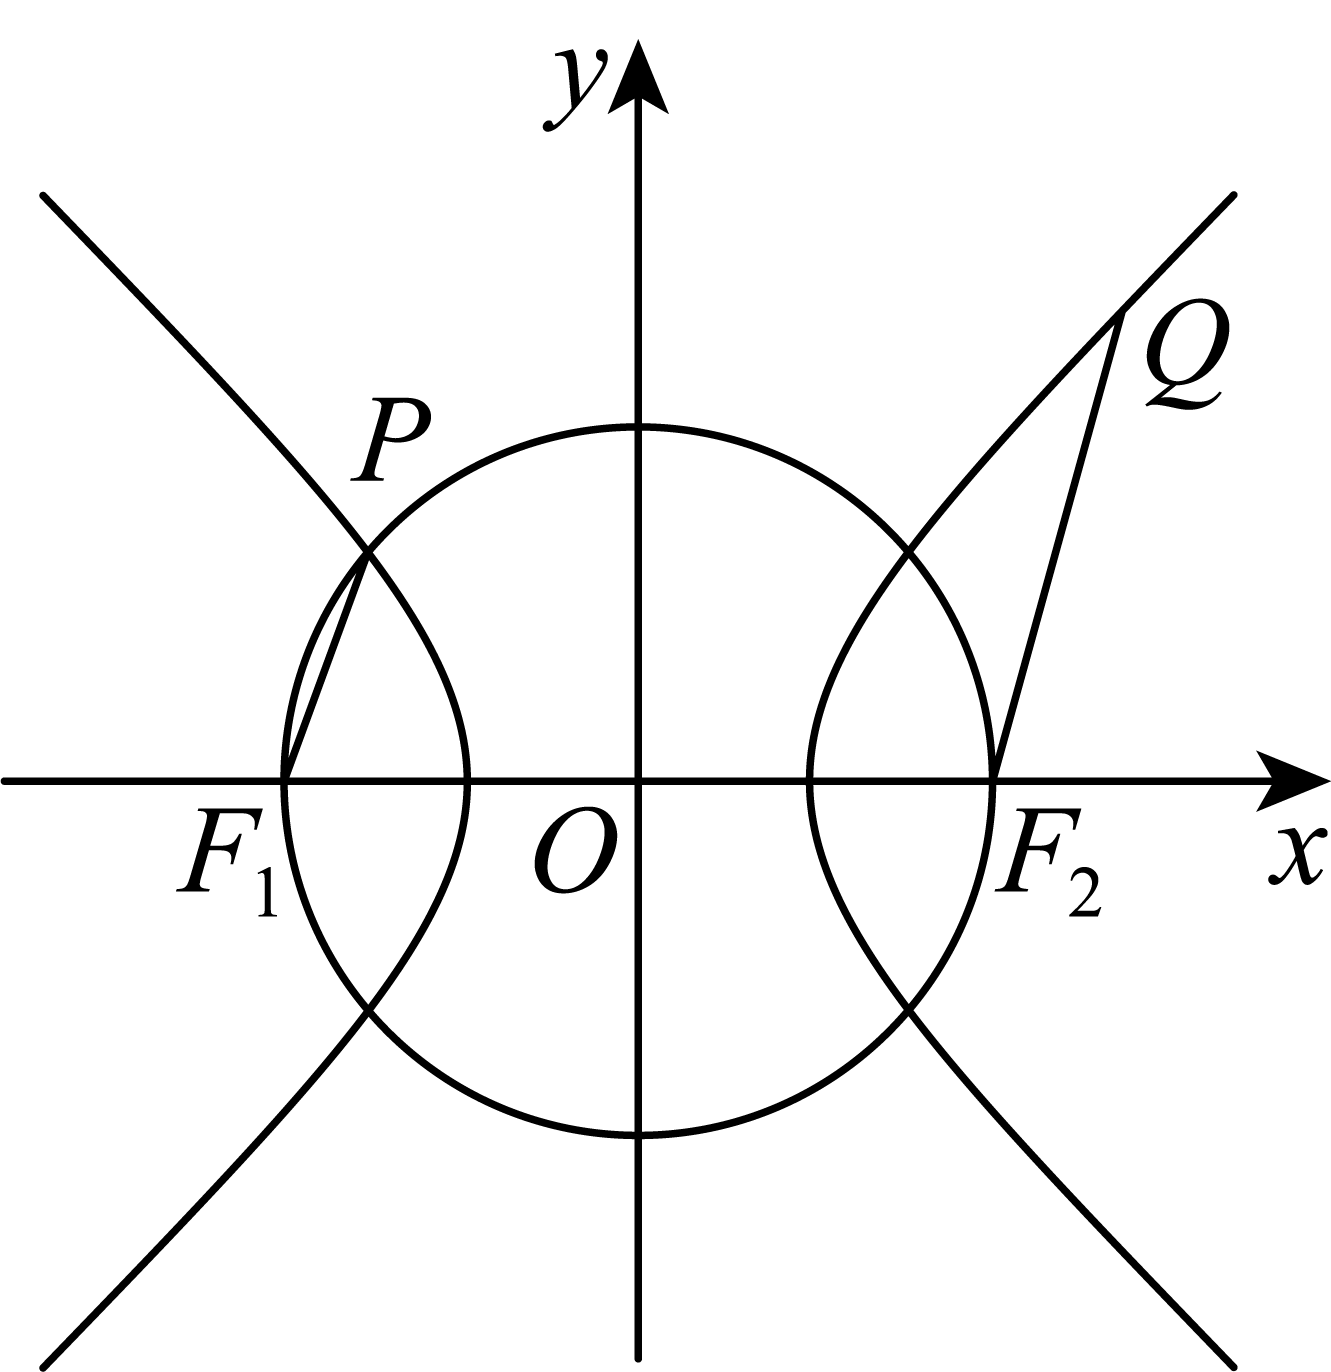
\includegraphics[width=36mm]{figs/14-拓04.png}}
\xiexwei{14mm}

\begin{ansblock}[2章-拓-课时14-18]
% ans:2章-拓-课时14-18
\ansitem{20}{曲线是双曲线（两支）：以 AB 所在直线为 x 轴、AB 中点为原点，其方程为 x²/9−y²/16=1。}
\ansnote{详解}{曲线上点\(P\)满足\(\bigl||PA|-|PB|\bigr|=6<|AB|=10\)，由定义轨迹为双曲线，\(2a=6\)、\(2c=10\)，\(a=3\)、\(c=5\)，\(b^{2}=25-9=16\)．以\(AB\)中点为原点、\(AB\)所在直线为\(x\)轴建系，方程为\(x^{2}/9-y^{2}/16=1\)．作图观察：交点连成两支光滑曲线，与双曲线吻合．}
\end{ansblock}

\liB{变式\textbf{21}}{简单(知识点二)}{}{设动点\(M\)到定点\(F(3,0)\)的距离与它到直线\(l\)：\(x=4/3\)的距离之比为\(3/2\)，求点\(M\)的轨迹方程．}
\xiexwei{14mm}

\begin{ansblock}[2章-拓-课时14-23]
% ans:2章-拓-课时14-23
\ansitem{21}{x²/4−y²/5=1。}
\ansnote{详解}{（直接法）设\(M(x,y)\)：\(\sqrt{(x-3)^{2}+y^{2}}=(3/2)\left|x-4/3\right|\)．两边平方：\(x^{2}-6x+9+y^{2}=(9/4)\left(x^{2}-(8/3)x+16/9\right)=(9/4)x^{2}-6x+4\)．\par\noindent \(-6x\)抵消：\(y^{2}=(9/4)x^{2}+4-x^{2}-9=(5/4)x^{2}-5\)，即\((5/4)x^{2}-y^{2}=5\)，标准形\(x^{2}/4-y^{2}/5=1\)．验算：\(a=2\)、\(c=3\)与准线位置\(x=a^{2}/c=4/3\)、比值\(c/a=3/2\)相容合．}
\ansnote{点睛}{本题源自“到定点与定直线距离之比为常数”的轨迹语境，该刻画属教材选学内容；未学者按上述直接法（设点、列距离等式、平方化简）可完整求解，无需引用第二定义．}
\end{ansblock}

\liB{变式\textbf{22}}{简单(知识点二)}{}{已知双曲线\(x^{2}/a^{2}-y^{2}/b^{2}=1\)（\(a>0\)，\(b>0\)）的左焦点为\(F(-c,0)\)，直线\(l\)：\(x=-a^{2}/c\)．设\(P\)是双曲线上的一点，求\(P\)到\(F\)的距离与\(P\)到直线\(l\)的距离之比．}
\xiexwei{14mm}

{\ansblockgrayfalse
\begin{ansblock}[2章-拓-课时14-24]
% ans:2章-拓-课时14-24
\ansitem{22}{比值等于 c/a（离心率 e）。}
\ansnote{详解}{（直接法）\(P(x,y)\)在双曲线上：\(y^{2}=b^{2}(x^{2}/a^{2}-1)\)．\(d_1=|PF|=\sqrt{(x+c)^{2}+y^{2}}\)，代入并用\(b^{2}=c^{2}-a^{2}\)化简：\(x^{2}+2cx+c^{2}+(c^{2}-a^{2})x^{2}/a^{2}-(c^{2}-a^{2})=(c^{2}/a^{2})x^{2}+2cx+a^{2}=\left[(c/a)x+a\right]^{2}\)．\par\noindent \(d_2=\left|x+a^{2}/c\right|\)（\(P\)到\(l\)的距离）．故\(d_1/d_2=(c/a)\left|x+a^{2}/c\right|/\left|x+a^{2}/c\right|=c/a\)（即离心率\(e\)）．}
\ansnote{点睛}{同上题：以准线措辞给出的距离比刻画属选学内容语境；未学者按直接法（配方化简上式）可完整求解，无需引用第二定义．}
\end{ansblock}}

\liB{变式\textbf{23}}{简单(知识点二)}{}{设动点\(M\)到定点\(F(-c,0)\)的距离与它到直线\(l\)：\(x=-a^{2}/c\)的距离之比为\(c/a\)，其中\(c>a>0\)，求点\(M\)的轨迹方程，并用得到的轨迹方程解释 2.6.2 中例 3 得到的结果．}
\xiexwei{14mm}

{\ansblockgrayfalse
\begin{ansblock}[2章-拓-课时14-27]
% ans:2章-拓-课时14-27
\ansitem{23}{x²/a²−y²/b²=1，其中 b²=c²−a²。}
\ansnote{详解}{（直接法）设\(M(x,y)\)：\(\sqrt{(x+c)^{2}+y^{2}}=(c/a)\left|x+a^{2}/c\right|\)．平方：\(x^{2}+2cx+c^{2}+y^{2}=(c^{2}/a^{2})x^{2}+2cx+a^{2}\)，\(2cx\)抵消：\(y^{2}=(c^{2}/a^{2}-1)x^{2}-(c^{2}-a^{2})=(b^{2}/a^{2})x^{2}-b^{2}\)（\(b^{2}=c^{2}-a^{2}\)），即\(x^{2}/a^{2}-y^{2}/b^{2}=1\)．解释：2.6.2 例 3 所得轨迹方程正是\(x^{2}/a^{2}-y^{2}/b^{2}=1\)（\(b^{2}=c^{2}-a^{2}\)），本题表明该双曲线可由“到定点与到定直线距离之比为常数\(c/a\)”直接刻画．}
\ansnote{点睛}{同上两题：距离比为常数\(c/a\;(>1)\)的轨迹即双曲线，属选学内容语境；未学者按直接法（平方化简）可完整求解，无需引用第二定义．}
\end{ansblock}}

\xiaojie{①识别：给渐近线与离心率之一反求另一、共渐近线系代点定参、由距离条件（点到直线距离、距离之比）定方程或轨迹的题，判归本题型.}
\bindp {\kaishu ②操作：\(e^{2}=1+(b/a)^{2}\)是渐近线与离心率互化的桥梁；距离比轨迹按直接法设点列式平方化简；距离恒等式\(d=b\)可作验算标尺.}
\bindp {\kaishu ③收束：未限焦点位置的离心率题两解并立；距离比\(c/a>1\)恒为双曲线轨迹，轨迹限定某支时补写坐标范围.}

% ---------- 探究点四 焦半径·最值·恒等与轨迹分类 ----------
\tjdnr{四}{焦半径·最值·恒等与轨迹分类}{例\textbf{24}}{中档(知识点三)}{已知双曲线\(x^{2}/a^{2}-y^{2}/b^{2}=1\)（\(a>0\)，\(b>0\)），\(M\)，\(N\)是双曲线上关于原点对称的两点，\(P\)是双曲线上的动点，直线\(PM\)，\(PN\)的斜率分别为\(k_1\)，\(k_2\)（\(k_1k_2\neq 0\)），若\(|k_1|+|k_2|\)的最小值为2，则双曲线的离心率为\nobreak(\kongwei)}

\bindopt {\fontsize{10.5pt}{\qpTJgLeadLiti}\selectfont \makebox[\dimexpr0.5\linewidth-1em\relax][l]{A．\(\sqrt{2}\)}\makebox[\dimexpr0.5\linewidth-1em\relax][l]{B．\(\sqrt{5}/2\)}\par}

\bindopt {\fontsize{10.5pt}{\qpTJgLeadLiti}\selectfont \makebox[\dimexpr0.5\linewidth-1em\relax][l]{C．\(\sqrt{3}/2\)}\makebox[\dimexpr0.5\linewidth-1em\relax][l]{D．\(3/2\)}\par}

{\ansblockgrayfalse
\begin{ansblock}[2章-练-课时14-12]
% ans:2章-练-课时14-12
\ansitem{24}{A}
\ansnote{详解}{设\(M(x_0,y_0)\)，则\(N(-x_0,-y_0)\)，\(P(x,y)\)（\(x\neq\pm x_0\)）．\(k_1k_2=\dfrac{y-y_0}{x-x_0}\cdot\dfrac{y+y_0}{x+x_0}=\dfrac{y^{2}-y_0^{2}}{x^{2}-x_0^{2}}\)（坐标点差法，不引名目）．\(M\)、\(P\)均在双曲线上：\(y^{2}=b^{2}(x^{2}/a^{2}-1)\)，\(y_0^{2}=b^{2}(x_0^{2}/a^{2}-1)\)，相减得\(y^{2}-y_0^{2}=(b^{2}/a^{2})(x^{2}-x_0^{2})\)，故\(k_1k_2=b^{2}/a^{2}\)（定值）．\par\noindent 于是\(|k_1|+|k_2|\geqslant 2\sqrt{|k_1k_2|}=2b/a\)（当\(|k_1|=|k_2|=b/a\)时取等，\(P\)可取到），由最小值2得\(b/a=1\)，\(e=\sqrt{1+(b/a)^{2}}=\sqrt{2}\)，故选A．}
\end{ansblock}}

\liB{变式\textbf{25}}{中档(知识点三)}{}{已知双曲线\(x^{2}/16-y^{2}/9=1\)的右焦点为\(F\)，且\(P\)是双曲线上一点，写出\(|PF|\)的最小值．}
\xiexwei{7mm}

\begin{ansblock}[2章-练-课时14-13]
% ans:2章-练-课时14-13
\ansitem{25}{1}
\ansnote{详解}{\(c^{2}=16+9=25\)，\(c=5\)，右焦点\(F(5,0)\)．设\(P(x,y)\)，\(|PF|^{2}=(x-5)^{2}+y^{2}\)．由\(y^{2}=9(x^{2}/16-1)\)（\(|x|\geqslant 4\)）：\(|PF|^{2}=x^{2}-10x+25+(9/16)x^{2}-9=(25/16)x^{2}-10x+16\)．对称轴\(x=10/(2\times 25/16)=16/5<4\)，故在\(|x|\geqslant 4\)上于\(x=4\)取最小：\(|PF|^{2}=(25/16)\times 16-40+16=1\)，\(|PF|_{\min}=1\)（即右顶点处取得，同支焦半径最小值\(c-a=5-4=1\)合）．}
\end{ansblock}

\tjdnr{四}{焦半径·最值·恒等与轨迹分类}{例\textbf{26}}{中档(知识点三)}{求证：双曲线的焦点到其渐近线的距离等于半虚轴长．}
\xiexwei{14mm}

{\ansblockgrayfalse
\begin{ansblock}[2章-练-课时14-14]
% ans:2章-练-课时14-14
\ansitem{26}{证明见解析。}
\ansnote{详解}{证明：不妨先设焦点在\(x\)轴：双曲线\(x^{2}/a^{2}-y^{2}/b^{2}=1\)（\(a>0\)，\(b>0\)），焦点\(F(c,0)\)，渐近线\(y=\pm(b/a)x\)，即\(bx\mp ay=0\)．焦点到渐近线的距离\(d=|bc-a\cdot 0|/\sqrt{a^{2}+b^{2}}=bc/c=b\)（半虚轴长）．\par\noindent 焦点在\(y\)轴时（\(y^{2}/a^{2}-x^{2}/b^{2}=1\)，焦点\(F(0,c)\)，渐近线\(y=\pm(a/b)x\)即\(ay\mp bx=0\)）：\(d=|a\cdot 0-bc|/\sqrt{a^{2}+b^{2}}=bc/c=b\)，等式仍成立．证毕．}
\end{ansblock}}

\liB{变式\textbf{27}}{简单(知识点三)}{}{已知\(P\)是双曲线\(x^{2}-y^{2}/3=1\)上一点，\(A(3,0)\)，求\(|PA|\)的最小值．}
\xiexwei{12mm}

\begin{ansblock}[2章-拓-课时14-22]
% ans:2章-拓-课时14-22
\ansitem{27}{2}
\ansnote{详解}{设\(P(x,y)\)（\(|x|\geqslant 1\)）：\(|PA|^{2}=(x-3)^{2}+y^{2}=(x-3)^{2}+3(x^{2}-1)=4x^{2}-6x+6\)．对称轴\(x=3/4<1\)，故\(x=1\)（右顶点）时取最小：\(4-6+6=4\)，\(|PA|_{\min}=2\)．}
\end{ansblock}

\tjdnr{四}{焦半径·最值·恒等与轨迹分类}{例\textbf{28}}{简单(知识点三)}{已知\(F_1\)，\(F_2\)是双曲线\(x^{2}/9-y^{2}/16=1\)的两个焦点，点\(M\)在双曲线上，如果\(MF_1\perp MF_2\)，求\(\triangle MF_1F_2\)的面积．}
\xiexwei{12mm}

\begin{ansblock}[2章-拓-课时14-25]
% ans:2章-拓-课时14-25
\ansitem{28}{16}
\ansnote{详解}{\(a=3\)，\(b=4\)，\(c=5\)．设两焦半径\(r_1=|MF_1|\)，\(r_2=|MF_2|\)（\(r_1>r_2\)）．\(MF_1\perp MF_2\)：\(r_1^{2}+r_2^{2}=|F_1F_2|^{2}=100\)；定义：\(r_1-r_2=2a=6\)．\par\noindent \((r_1-r_2)^{2}=100-2r_1r_2=36\)，得\(r_1r_2=32\)．\(S=(1/2)r_1r_2\sin 90^{\circ}=16\)．}
\end{ansblock}

\liB{变式\textbf{29}}{简单(知识点三)}{}{如果过点\((6,0)\)的直线与过点\((-6,0)\)的直线相交于点\(M\)，而且两直线斜率的乘积为\(a\)，其中\(a\neq 0\)．(1)求点\(M\)的轨迹方程；(2)讨论\(M\)的轨迹是何种曲线．}
\xiexwei{14mm}

{\ansblockgrayfalse
\begin{ansblock}[2章-拓-课时14-26]
% ans:2章-拓-课时14-26
\ansitem{29}{(1) ax²−y²=36a（y≠0）；(2) a>0 时为焦点在 x 轴的双曲线（除去顶点）；a<0 时为椭圆：其中 a=−1 为圆 x²+y²=36（y≠0），−1<a<0 为焦点在 x 轴的椭圆，a<−1 为焦点在 y 轴的椭圆（均除去长轴端点——方程中 y≠0）。}
\ansnote{详解}{(1)过\((6,0)\)斜率\(k_1\)、过\((-6,0)\)斜率\(k_2\)，\(k_1k_2=a\)．设\(M(x,y)\)：\(k_1=y/(x-6)\)，\(k_2=y/(x+6)\)（\(x\neq\pm 6\)，且\(M\)不与\((\pm 6,0)\)重合故\(y\neq 0\)）．\([y/(x-6)]\cdot[y/(x+6)]=a\)，得\(y^{2}=a(x^{2}-36)\)，即\(ax^{2}-y^{2}=36a\)（\(y\neq 0\)）．\par\noindent (2)\(a>0\)：\(x^{2}/36-y^{2}/(36a)=1\)，焦点在\(x\)轴的双曲线（除去顶点）；\(a<0\)：记\(a=-|a|\)，\(x^{2}/36+y^{2}/(36|a|)=1\)，椭圆；其中\(a=-1\)：\(x^{2}+y^{2}=36\)，圆；\(-1<a<0\)：\(36>36|a|\)，焦点在\(x\)轴的椭圆；\(a<-1\)：\(36<36|a|\)，焦点在\(y\)轴的椭圆（均除去\(x\)轴上的点，即\(y\neq 0\)）．}
\end{ansblock}}

\liB{变式\textbf{30}}{中档(知识点三)}{}{设等轴双曲线\(C\)的中心为\(O\)，焦点为\(F_1\)，\(F_2\)，\(P\)为\(C\)上任意一点，求证：\(|PO|^{2}=|PF_1|\cdot|PF_2|\)．}
\xiexwei{14mm}

{\ansblockgrayfalse
\begin{ansblock}[2章-拓-课时14-08]
% ans:2章-拓-课时14-08
\ansitem{30}{证明见解析。}
\ansnote{详解}{证明：设\(C\)：\(x^{2}/m^{2}-y^{2}/m^{2}=1\)（\(m>0\)），则\(F_1(-\sqrt{2}m,0)\)，\(F_2(\sqrt{2}m,0)\)．设\(P(x,y)\)，满足\(x^{2}-y^{2}=m^{2}\)．\(|PO|^{2}=x^{2}+y^{2}\)．\par\noindent \(|PF_1|\cdot|PF_2|=\sqrt{(x+\sqrt{2}m)^{2}+y^{2}}\cdot\sqrt{(x-\sqrt{2}m)^{2}+y^{2}}\)，根号内合并为\(\sqrt{(x^{2}+2m^{2}+y^{2})^{2}-8m^{2}x^{2}}\)．用\(y^{2}=x^{2}-m^{2}\)化简：\(x^{2}+2m^{2}+y^{2}=2x^{2}+m^{2}\)，\((2x^{2}+m^{2})^{2}-8m^{2}x^{2}=4x^{4}-4m^{2}x^{2}+m^{4}=(2x^{2}-m^{2})^{2}\)．\par\noindent 故\(|PF_1|\cdot|PF_2|=|2x^{2}-m^{2}|=2x^{2}-m^{2}\)（\(|x|\geqslant m\)时为正）\(=x^{2}+y^{2}=|PO|^{2}\)．证毕．验算：\(m=1\)，\(P(\sqrt{2},1)\)：\(|PO|^{2}=3\)，\(|PF_1|=3\)，\(|PF_2|=1\)，积为3合．}
\end{ansblock}}

\xiaojie{①识别：焦半径最值、焦点三角形面积与垂直、距离/数量积恒等证明、斜率积轨迹及曲线类型分类的题，判归本题型；工具链为定义＋勾股＋消元配方.}
\bindp {\kaishu ②操作：同支焦半径\(|PF|_{\min}=c-a\)在顶点取得，消元后按\(x\)范围取端点；焦点三角形用\(r_1-r_2=2a\)与勾股联立；斜率积用点差法定值再分类讨论.}
\bindp {\kaishu ③收束：轨迹题挖去与定点重合的点（\(y\neq 0\)）须保留在方程与结论中；分类讨论按参数与临界值比较，逐类指明曲线类型与焦点位置.}

% ---------- 探究点五 模型求e与实际应用 ----------
\tjdnr{五}{模型求e与实际应用}{例\textbf{31}}{中档(知识点一)}{过双曲线\(x^{2}/a^{2}-y^{2}/b^{2}=1\)的右焦点\(F_2\)作垂直于实轴的弦\(PQ\)，\(F_1\)是左焦点，若\(\angle PF_1Q=90^{\circ}\)，则双曲线的离心率是\nobreak(\kongwei)}

\bindopt {\fontsize{10.5pt}{\qpTJgLeadLiti}\selectfont \makebox[\dimexpr0.5\linewidth-1em\relax][l]{A．\(\sqrt{2}\)}\makebox[\dimexpr0.5\linewidth-1em\relax][l]{B．\(1+\sqrt{2}\)}\par}

\bindopt {\fontsize{10.5pt}{\qpTJgLeadLiti}\selectfont \makebox[\dimexpr0.5\linewidth-1em\relax][l]{C．\(2+\sqrt{2}\)}\makebox[\dimexpr0.5\linewidth-1em\relax][l]{D．\(3-\sqrt{2}\)}\par}

\begin{ansblock}[2章-拓-课时14-01]
% ans:2章-拓-课时14-01
\ansitem{31}{B}
\ansnote{详解}{\(PQ\)为通径，\(P(c,\pm b^{2}/a)\)，\(|PQ|=2b^{2}/a\)．\(\triangle PF_1Q\)中\(\angle PF_1Q=90^{\circ}\)，\(F_2\)为斜边\(PQ\)的中点，由直角三角形斜边中线定理\(|F_1F_2|=|PQ|/2\)，即\(2c=b^{2}/a\)，\(2ac=b^{2}=c^{2}-a^{2}\)．两边除以\(a^{2}\)：\(e^{2}-2e-1=0\)，\(e>1\)，\(e=1+\sqrt{2}\)，故选B．}
\end{ansblock}

\liB{变式\textbf{32}}{难(知识点一)}{}{已知双曲线\(C\)：\(x^{2}/a^{2}-y^{2}/b^{2}=1\)（\(a>0\)，\(b>0\)）的左、右焦点分别为\(F_1\)，\(F_2\)，过\(F_1\)的直线与\(C\)的两条渐近线分别交于\(A\)，\(B\)两点．若\(|F_1A|=|AB|\)，\(\overrightarrow{F_1B}\cdot\overrightarrow{F_2B}=0\)，则\(C\)的离心率为\kongbai{}．}
\xiexwei{7mm}

{\ansblockgrayfalse
\begin{ansblock}[2章-拓-课时14-02]
% ans:2章-拓-课时14-02
\ansitem{32}{2}
\ansnote{详解}{\(A\)在线段\(F_1B\)上且\(|F_1A|=|AB|\)，故\(A\)为\(F_1B\)的中点；\(O\)为\(F_1F_2\)的中点，故\(OA\)是\(\triangle F_1F_2B\)的中位线：\(OA\parallel F_2B\)，\(|F_2B|=2|OA|\)．\par\noindent 由\(\overrightarrow{F_1B}\cdot\overrightarrow{F_2B}=0\)得\(F_1B\perp F_2B\)，结合\(OA\parallel F_2B\)得\(OA\perp F_1B\)．于是\(\triangle F_1OB\)中，\(OA\)既是边\(F_1B\)上的中线又是高，故\(\triangle F_1OB\)等腰：\(|OB|=|OF_1|=c\)，且\(\angle AOF_1=\angle AOB\)．\par\noindent 又\(A\)、\(B\)分别在两条渐近线上，两渐近线关于\(x\)轴对称，故\(\angle BOF_2=\angle AOF_1\)；而\(\angle AOF_1+\angle AOB+\angle BOF_2=180^{\circ}\)，三者在上述等量关系下相等，各为\(60^{\circ}\)．故\(b/a=\tan 60^{\circ}=\sqrt{3}\)，\(e=\sqrt{1+(b/a)^{2}}=\sqrt{1+3}=2\)．}
\end{ansblock}}

\tjdnr{五}{模型求e与实际应用}{例\textbf{33}}{中档(知识点一)}{已知\(F_1\)，\(F_2\)是双曲线\(x^{2}/a^{2}-y^{2}/b^{2}=1\)（\(a>0\)，\(b>0\)）的左、右焦点，以\(F_1F_2\)为直径的圆与双曲线交于不同的四点，顺次连接焦点和这四点恰好组成一个正六边形，则该双曲线的离心率为\nobreak(\kongwei)}

\bindopt {\fontsize{10.5pt}{\qpTJgLeadLiti}\selectfont \makebox[\dimexpr0.5\linewidth-1em\relax][l]{A．\(\sqrt{2}\)}\makebox[\dimexpr0.5\linewidth-1em\relax][l]{B．\(\sqrt{3}\)}\par}

\bindopt {\fontsize{10.5pt}{\qpTJgLeadLiti}\selectfont \makebox[\dimexpr0.5\linewidth-1em\relax][l]{C．\(\sqrt{3}+1\)}\makebox[\dimexpr0.5\linewidth-1em\relax][l]{D．\((\sqrt{5}+1)/2\)}\par}

\begin{ansblock}[2章-拓-课时14-03]
% ans:2章-拓-课时14-03
\ansitem{33}{C}
\ansnote{详解}{六个顶点内接于以\(F_1F_2\)为直径的圆，由直径所对圆周角\(\angle F_1PF_2=90^{\circ}\)；正六边形各边对圆心角\(60^{\circ}\)，得\(\angle PF_2F_1=30^{\circ}\)．解三角形：\(|PF_2|=2c\cos 30^{\circ}=\sqrt{3}c\)，\(|PF_1|=2c\sin 30^{\circ}=c\)．\(P\)在双曲线上，\(|PF_2|-|PF_1|=2a\)，即\(\sqrt{3}c-c=2a\)，\(e=c/a=2/(\sqrt{3}-1)=\sqrt{3}+1\)，故选C．}
\end{ansblock}

\liB{变式\textbf{34}}{难(知识点一)}{}{如图，\(F_1\)，\(F_2\)分别是双曲线\(x^{2}/a^{2}-y^{2}/b^{2}=1\)（\(a>0\)，\(b>0\)）的左、右焦点，点\(P\)是双曲线与圆\(x^{2}+y^{2}=a^{2}+b^{2}\)在第二象限的一个交点，点\(Q\)在双曲线上，且\(\overrightarrow{F_1P}=(1/2)\overrightarrow{F_2Q}\)，则双曲线的离心率为\nobreak(\kongwei)}
\ansfig{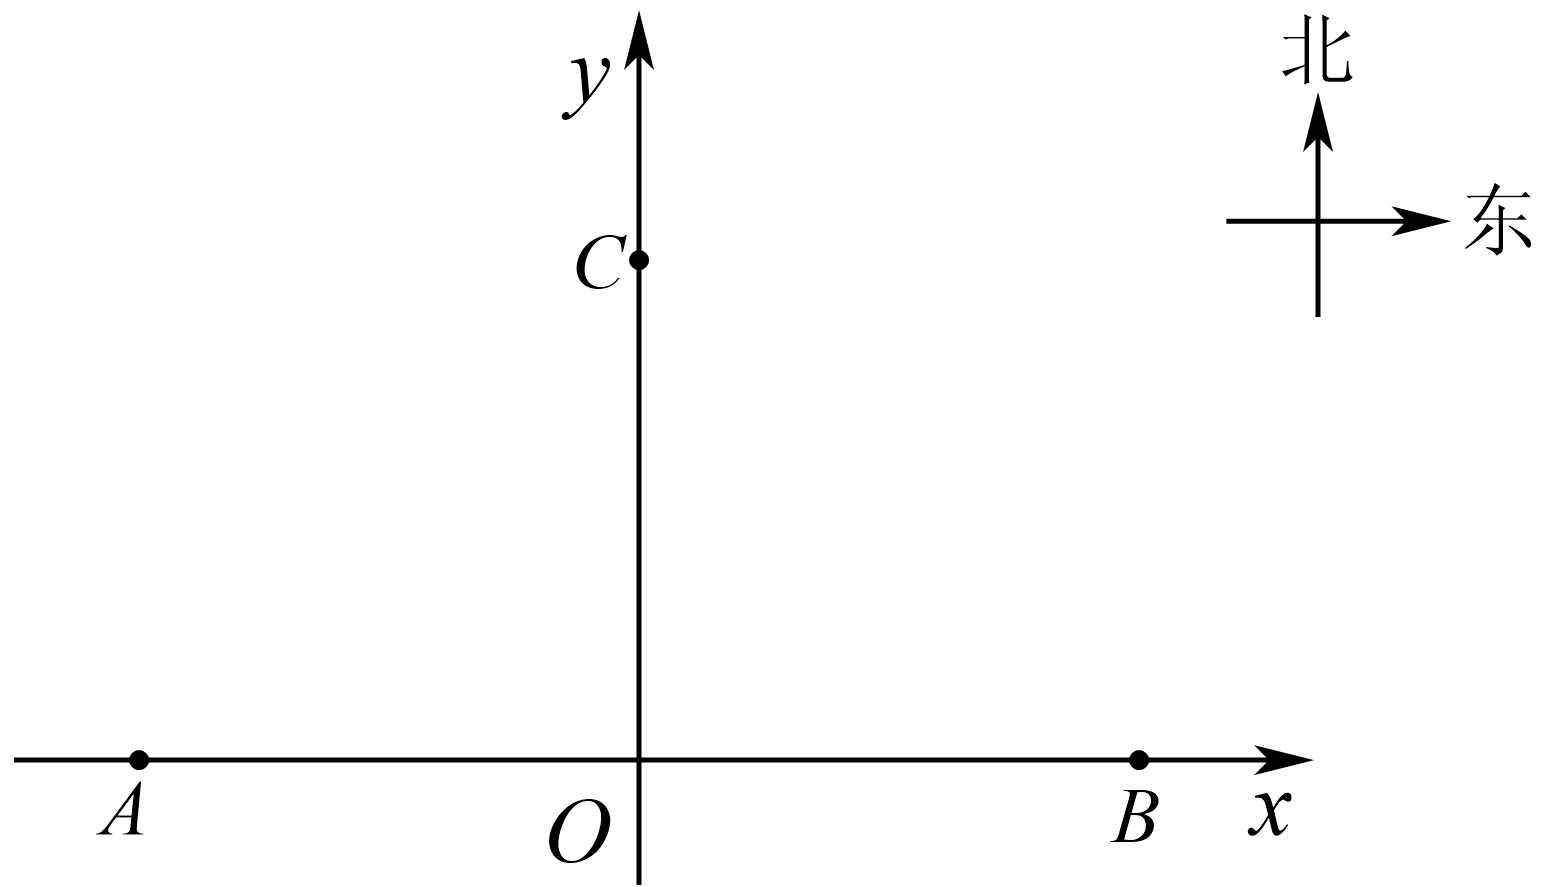
\includegraphics[width=40mm]{figs/14-拓11.png}}

\bindopt {\fontsize{10.5pt}{\qpTJgLeadLiti}\selectfont \makebox[\dimexpr0.5\linewidth-1em\relax][l]{A．\(\sqrt{10}/2\)}\makebox[\dimexpr0.5\linewidth-1em\relax][l]{B．\(\sqrt{2}\)}\par}

\bindopt {\fontsize{10.5pt}{\qpTJgLeadLiti}\selectfont \makebox[\dimexpr0.5\linewidth-1em\relax][l]{C．\(\sqrt{3}\)}\makebox[\dimexpr0.5\linewidth-1em\relax][l]{D．\(\sqrt{17}/3\)}\par}

{\ansblockgrayfalse
\begin{ansblock}[2章-拓-课时14-04]
% ans:2章-拓-课时14-04
\ansitem{34}{D}
\ansnote{详解}{圆\(x^{2}+y^{2}=a^{2}+b^{2}\)的半径为\(c\)，其直径恰为\(F_1F_2\)，故\(P\)在圆上，\(\angle F_1PF_2=90^{\circ}\)（直径所对圆周角）．设\(|PF_1|=n\)，由定义\(|PF_2|=2a+n\)．Rt\(\triangle PF_1F_2\)中：\(n^{2}+(2a+n)^{2}=4c^{2}\)，展开得\(n^{2}=2b^{2}-2an\)．\par\noindent 由\(\overrightarrow{F_1P}=(1/2)\overrightarrow{F_2Q}\)（同向向量）得\(|F_2Q|=2n\)，且\(F_1P\parallel F_2Q\)，故\(\angle QF_2F_1=180^{\circ}-\angle PF_1F_2\)，\(\cos\angle QF_2F_1=-n/(2c)\)．由定义\(|F_1Q|=2a+2n\)，\(\triangle F_1F_2Q\)中余弦定理：\((2a+2n)^{2}=(2n)^{2}+(2c)^{2}+4n^{2}\)，化简得\(2an=b^{2}+n^{2}\)，即\(b^{2}=2an-n^{2}\)．\par\noindent 与\(n^{2}=2b^{2}-2an\)联立：\(3n^{2}=2an\)，\(a=(3/2)n\)；\(b^{2}=2n^{2}\)，\(c^{2}=(17/4)n^{2}\)，\(e=c/a=\sqrt{17}/3\)，故选D．}
\end{ansblock}}

\tjdnr{五}{模型求e与实际应用}{例\textbf{35}}{中档(知识点一)}{已知双曲线\(C\)：\(x^{2}/a^{2}-y^{2}/b^{2}=1\)（\(a>0\)，\(b>0\)）的左、右顶点分别为\(A\)，\(B\)，圆\(P\)：\(x^{2}+(y-a)^{2}=2a^{2}\)与双曲线\(C\)在第一象限的交点为\(M\)，记直线\(MA\)，\(MB\)的斜率分别为\(m\)，\(n\)，且\(n-m=3\)，则双曲线的离心率为\kongbai{}．}
\xiexwei{7mm}

{\ansblockgrayfalse
\begin{ansblock}[2章-拓-课时14-05]
% ans:2章-拓-课时14-05
\ansitem{35}{√3}
\ansnote{详解}{\(O(0,0)\)，\(A(-a,0)\)，\(B(a,0)\)，圆\(P\)的圆心为\(P(0,a)\)，半径\(\sqrt{2}a\)．\(|OA|=|OB|=|OP|=a\)，故\(O\)、\(A\)、\(P\)、\(B\)四点共圆（圆心\(O\)、半径\(a\)），其中\(AB\)为该圆的直径，\(P\)在圆上，由直径所对圆周角得\(\angle APB=90^{\circ}\)．\(M\)在圆上且在第一象限，位于弦\(AB\)所对优弧，故\(\angle AMB=(1/2)\angle APB=45^{\circ}\)．\par\noindent 夹角公式：\(\tan\angle AMB=(n-m)/(1+nm)=1\)，\(n-m=3\)，得\(nm=2\)．设\(M(x,y)\)：\(m=y/(x+a)\)，\(n=y/(x-a)\)，\(nm=y^{2}/(x^{2}-a^{2})\)；由\(y^{2}=b^{2}(x^{2}/a^{2}-1)\)得\(nm=b^{2}/a^{2}=2\)．\(e^{2}=1+b^{2}/a^{2}=3\)，\(e=\sqrt{3}\)．}
\end{ansblock}}

\liB{变式\textbf{36}}{中档(知识点一)}{}{\(l\)是经过双曲线\(C\)：\(x^{2}/a^{2}-y^{2}/b^{2}=1\)（\(a>0\)，\(b>0\)）焦点\(F\)且与实轴垂直的直线，\(A\)，\(B\)是双曲线\(C\)的两个顶点，若在\(l\)上存在一点\(P\)，使\(\angle APB=60^{\circ}\)，则双曲线离心率的最大值为\kongbai{}．}
\xiexwei{7mm}

{\ansblockgrayfalse
\begin{ansblock}[2章-拓-课时14-06]
% ans:2章-拓-课时14-06
\ansitem{36}{2√3/3}
\ansnote{详解}{设\(A(a,0)\)，\(B(-a,0)\)，\(P(c,y)\)（\(l\)：\(x=c\)）．\(k_{PA}=y/(c-a)\)，\(k_{PB}=y/(c+a)\)．由夹角公式\(\tan\angle APB=\left|[k_{PA}-k_{PB}]/[1+k_{PA}k_{PB}]\right|=\sqrt{3}\)：\(\left|(2ay)/(c^{2}-a^{2})\right|/\left|1+y^{2}/(c^{2}-a^{2})\right|=\sqrt{3}\)，整理为关于\(y\)的方程\(\sqrt{3}y^{2}-2ay+\sqrt{3}(c^{2}-a^{2})=0\)有实根．判别式\(\Delta=4a^{2}-12(c^{2}-a^{2})=4(4a^{2}-3c^{2})\geqslant 0\)，得\(e^{2}\leqslant 4/3\)，\(e\leqslant 2\sqrt{3}/3\)．离心率最大值\(2\sqrt{3}/3\)．验算：\(e=2\sqrt{3}/3\)时\(\Delta=0\)，\(P\)取对称轴位置\(y=a/\sqrt{3}\)合．}
\end{ansblock}}

\liB{变式\textbf{37}}{中档(知识点三)}{}{已知\(F_1\)，\(F_2\)为双曲线\(C\)：\(x^{2}/16-y^{2}/9=1\)的两个焦点，\(P\)，\(Q\)为\(C\)上关于坐标原点对称的两点，且\(|PQ|=|F_1F_2|\)，则四边形\(PF_1QF_2\)的面积为\kongbai{}．}
\xiexwei{7mm}

\begin{ansblock}[2章-拓-课时14-09]
% ans:2章-拓-课时14-09
\ansitem{37}{18}
\ansnote{详解}{\(PQ\)与\(F_1F_2\)互相平分（\(P\)、\(Q\)关于\(O\)对称，\(F_1\)、\(F_2\)关于\(O\)对称）且\(|PQ|=|F_1F_2|\)，对角线相等又互相平分，故四边形\(PF_1QF_2\)为矩形，其面积\(=|PF_1|\cdot|PF_2|\)．矩形中\(|PF_1|^{2}+|PF_2|^{2}=|F_1F_2|^{2}=4c^{2}=100\)；又\(\bigl||PF_1|-|PF_2|\bigr|=2a=8\)．故\(2|PF_1||PF_2|=100-64=36\)，\(|PF_1||PF_2|=18\)，面积18．}
\end{ansblock}

\liB{变式\textbf{38}}{中档(知识点三)}{}{若坐标原点\(O\)和点\(F(-2,0)\)分别为双曲线\(x^{2}/a^{2}-y^{2}=1\)（\(a>0\)）的中心和左焦点，点\(P\)为双曲线右支上的任意一点，则\(\overrightarrow{OP}\cdot\overrightarrow{FP}\)的最小值为\kongbai{}．}
\xiexwei{7mm}

\begin{ansblock}[2章-拓-课时14-10]
% ans:2章-拓-课时14-10
\ansitem{38}{3+2√3}
\ansnote{详解}{左焦点\((-\sqrt{a^{2}+1},0)=(-2,0)\)，得\(a^{2}=3\)．设\(P(x_0,y_0)\)（右支\(x_0\geqslant\sqrt{3}\)），\(y_0^{2}=x_0^{2}/3-1\)．\(\overrightarrow{OP}\cdot\overrightarrow{FP}=(x_0,y_0)\cdot(x_0+2,y_0)=x_0^{2}+2x_0+y_0^{2}=(4/3)x_0^{2}+2x_0-1\)．在\([\sqrt{3},+\infty)\)上单调递增，\(x_0=\sqrt{3}\)时取最小：\((4/3)\times 3+2\sqrt{3}-1=3+2\sqrt{3}\)．}
\end{ansblock}

\tjdnr{五}{模型求e与实际应用}{例\textbf{39}}{中档(知识点三)}{如图，某野生保护区监测中心设置在点\(O\)处，正西、正东、正北处有3个监测点\(A\)，\(B\)，\(C\)，且\(|OA|=|OB|=|OC|=30\)km，一名野生动物观察员在保护区遇险，发出求救信号，3个监测点均收到求救信号，\(A\)点接收到信号的时间比\(B\)点接收到信号的时间早\((40/V_0)\)s（注：信号每秒传播\(V_0\)km）.(1)求观察员所有可能出现的位置的轨迹方程；(2)若\(C\)点信号失灵，现立即以\(C\)为圆心进行“圆形”红外扫描，为保证有救援希望，扫描半径\(r\)至少是多少千米？}
\ansfig{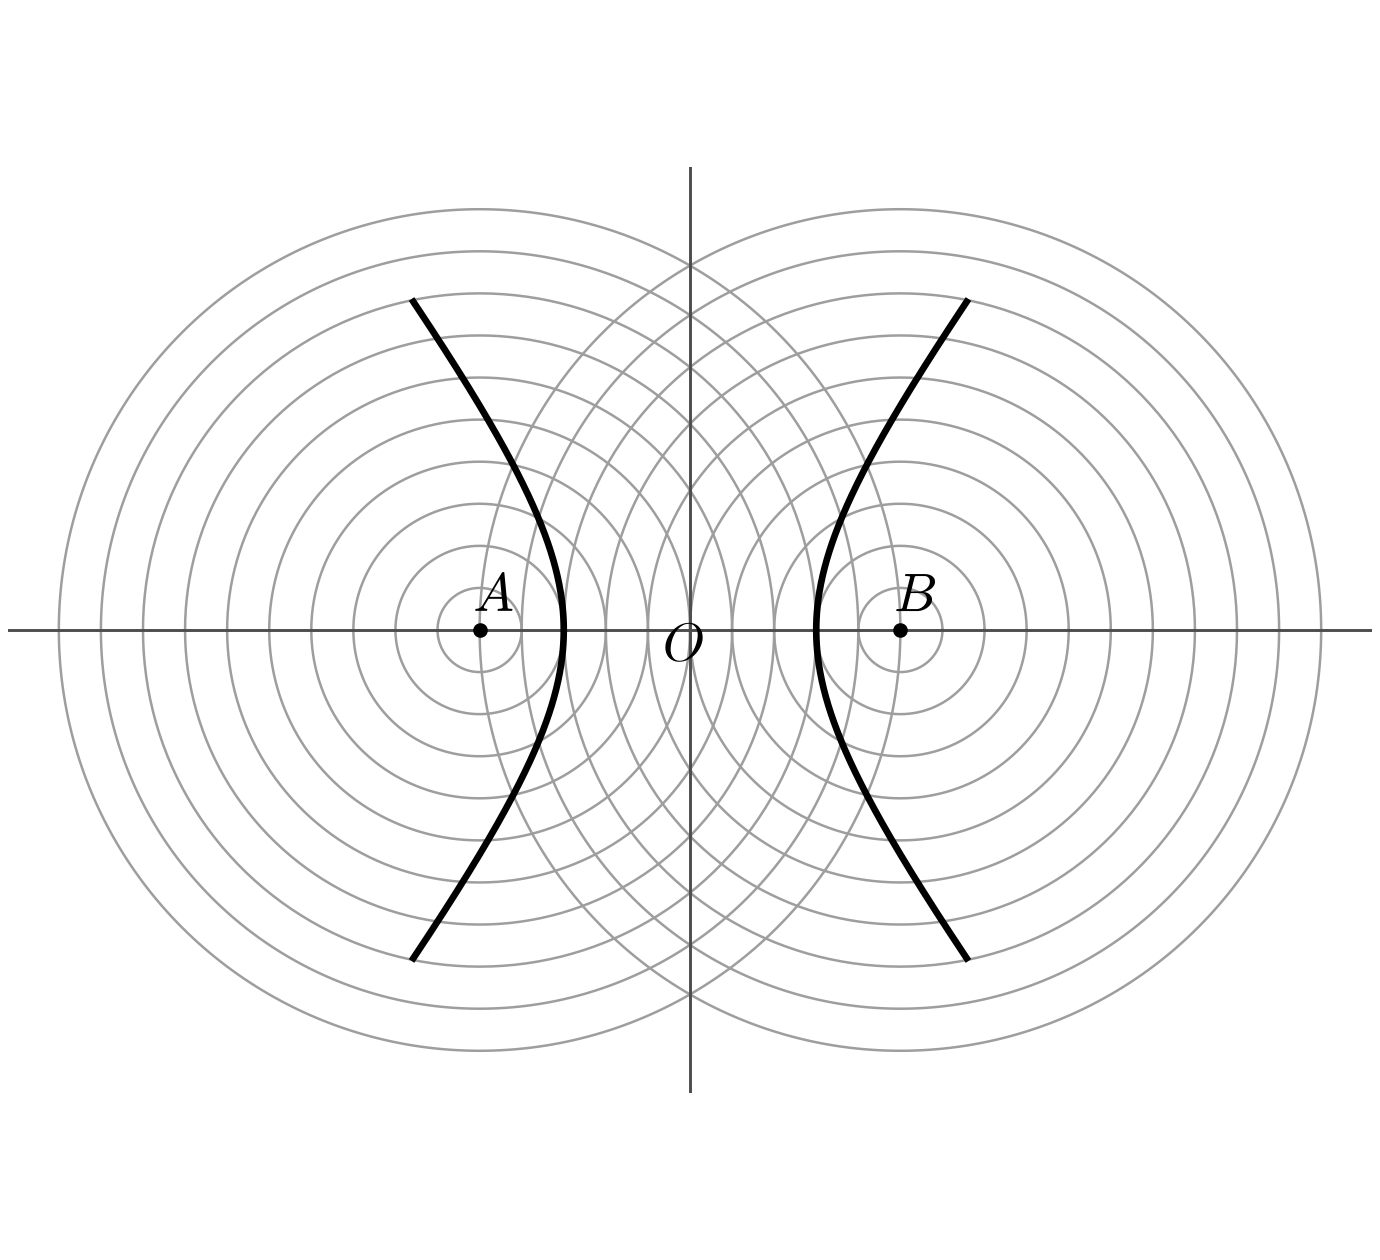
\includegraphics[width=38mm]{figs/14-拓18.png}}
\xiexwei{14mm}

{\ansblockgrayfalse
\begin{ansblock}[2章-拓-课时14-11]
% ans:2章-拓-课时14-11
\ansitem{39}{(1) x²/400−y²/500=1（x<0）；(2) 20√2 km。}
\ansnote{详解}{(1)以\(O\)为原点、\(AB\)所在直线为\(x\)轴建系：\(A(-30,0)\)，\(B(30,0)\)，\(C(0,30)\)．设观察员位置\(P(x,y)\)：\(|PB|-|PA|=(40/V_0)\cdot V_0=40<|AB|=60\)，轨迹为双曲线左支．\(2a=40\)，\(2c=60\)，\(a=20\)，\(c=30\)，\(b^{2}=c^{2}-a^{2}=500\)，轨迹方程\(x^{2}/400-y^{2}/500=1\)（\(x<0\)）．\par\noindent (2)设轨迹上一点\(M(x,y)\)：\(|MC|^{2}=x^{2}+(y-30)^{2}=x^{2}+y^{2}-60y+900\)．由\(x^{2}=(4/5)y^{2}+400\)：\(|MC|^{2}=(9/5)y^{2}-60y+1300=(9/5)(y-50/3)^{2}+800\geqslant 800\)．当\(y=50/3\)时\(|MC|_{\min}=20\sqrt{2}\)，扫描半径\(r\)至少\(20\sqrt{2}\) km．}
\end{ansblock}}

\liB{变式\textbf{40}}{中档(知识点二)}{\duoxuan\hspace{0.6em}}{定义：以双曲线的实轴为虚轴，虚轴为实轴的双曲线与原双曲线互为共轭双曲线．以下关于共轭双曲线的结论正确的是\nobreak(\kongwei)}

\lxopt{A．与\(x^{2}/a^{2}-y^{2}/b^{2}=1\)（\(a>0\)，\(b>0\)）共轭的双曲线是\(y^{2}/a^{2}-x^{2}/b^{2}=1\)（\(a>0\)，\(b>0\)）}

\lxopt{B．互为共轭的双曲线渐近线不相同}

\lxopt{C．互为共轭的双曲线的离心率为\(e_1\)、\(e_2\)，则\(e_1e_2\geqslant 2\)}

\lxopt{D．互为共轭的双曲线的4个焦点在同一圆上}

{\ansblockgrayfalse
\begin{ansblock}[2章-拓-课时14-12]
% ans:2章-拓-课时14-12
\ansitem{40}{CD}
\ansnote{详解}{A：按定义实虚轴互换，共轭双曲线应为\(y^{2}/b^{2}-x^{2}/a^{2}=1\)，A错；B：原曲线渐近线\(y=\pm(b/a)x\)，共轭曲线（\(y\)轴型）渐近线\(y=\pm(b/a)x\)（\(a/b\)与\(b/a\)互换后方程相同），渐近线相同，B错；C：\(e_1=c/a\)，\(e_2=c/b\)，\(e_1e_2=c^{2}/(ab)=(a^{2}+b^{2})/(ab)=a/b+b/a\geqslant 2\)（当且仅当\(a=b\)取等），C对；D：焦点\((\pm c,0)\)与\((0,\pm c)\)均在圆\(x^{2}+y^{2}=c^{2}\)上，D对．故选CD．}
\end{ansblock}}

\tjdnr{五}{模型求e与实际应用}{例\textbf{41}}{简单(知识点一)}{已知双曲线\(x^{2}/a^{2}-y^{2}=1\)（\(a>0\)）上关于原点对称的两个点\(P\)，\(Q\)，右顶点为\(A\)，线段\(AP\)的中点为\(E\)，直线\(QE\)交\(x\)轴于\(M(1,0)\)，则双曲线的离心率为\nobreak(\kongwei)}

\bindopt {\fontsize{10.5pt}{\qpTJgLeadLiti}\selectfont \makebox[\dimexpr0.5\linewidth-1em\relax][l]{A．\(\sqrt{5}\)}\makebox[\dimexpr0.5\linewidth-1em\relax][l]{B．\(\sqrt{5}/3\)}\par}

\bindopt {\fontsize{10.5pt}{\qpTJgLeadLiti}\selectfont \makebox[\dimexpr0.5\linewidth-1em\relax][l]{C．\(\sqrt{10}\)}\makebox[\dimexpr0.5\linewidth-1em\relax][l]{D．\(\sqrt{10}/3\)}\par}

\begin{ansblock}[2章-拓-课时14-32-1]
% ans:2章-拓-课时14-32-1
\ansitem{41}{D}
\ansnote{详解}{设\(P(x_0,y_0)\)、\(Q(-x_0,-y_0)\)，\(\triangle APQ\)三顶点纵坐标和为\(y_0-y_0+0=0\)，坐标和为\((a,0)\)，其重心为\(G(a/3,0)\)．重心在每条中线上，故\(G\)在中线\(QE\)上；\(QE\)与\(x\)轴的交点唯一，故\(M(1,0)\)即重心：\(a/3=1\)，\(a=3\)．\(b^{2}=1\)，\(c=\sqrt{9+1}=\sqrt{10}\)，\(e=c/a=\sqrt{10}/3\)，故选D．}
\end{ansblock}

\liB{变式\textbf{42}}{简单(知识点三)}{}{已知双曲线\(C\)：\(x^{2}/a^{2}-y^{2}/b^{2}=1\)（\(a>0\)，\(b>0\)）离心率为2，\(A\)、\(B\)分别为左、右顶点，点\(P\)为双曲线\(C\)在第一象限内的任意一点，点\(O\)为坐标原点，若\(PA\)、\(PB\)、\(PO\)的斜率分别为\(k_1\)、\(k_2\)、\(k_3\)，设\(m=k_1\cdot k_2\cdot k_3\)，则\(m\)的取值范围为\kongbai{}．}
\xiexwei{7mm}

\begin{ansblock}[2章-拓-课时14-32-2]
% ans:2章-拓-课时14-32-2
\ansitem{42}{(0, 3√3)}
\ansnote{详解}{\(e=2\)，\(c^{2}=4a^{2}\)，\(b^{2}=c^{2}-a^{2}=3a^{2}\)，\(b/a=\sqrt{3}\)．\(k_1k_2=\left[y_0/(x_0+a)\right]\cdot\left[y_0/(x_0-a)\right]=y_0^{2}/(x_0^{2}-a^{2})=(b^{2}/a^{2})(x_0^{2}-a^{2})/(x_0^{2}-a^{2})=b^{2}/a^{2}=3\)（坐标点差法，同例24）．\(P\)在第一象限右支：\(k_3=y_0/x_0\in(0,b/a)=(0,\sqrt{3})\)（\(P\)趋近顶点时\(k_3\to 0\)，沿渐近线方向\(k_3\to\sqrt{3}\)）．故\(m=3k_3\in(0,3\sqrt{3})\)．}
\end{ansblock}

\tjdnr{五}{模型求e与实际应用}{例\textbf{43}}{中档(知识点三)}{平面上一台机器人在运行中始终保持到点\(P(-2,0)\)的距离比到点\(Q(2,0)\)的距离大2，若机器人接触不到过点\(M(\sqrt{3},3)\)且斜率为\(k\)的直线，则\(k\)的取值范围是\kongbai{}．}
\xiexwei{7mm}

{\ansblockgrayfalse
\begin{ansblock}[2章-拓-课时14-33-1]
% ans:2章-拓-课时14-33-1
\ansitem{43}{[√3, 2√3)}
\ansnote{详解}{机器人到\(P\)的距离比到\(Q\)大2：距离差\(2<|PQ|=4\)，且距\(P\)更远，轨迹为双曲线右支：\(a=1\)，\(c=2\)，\(b^{2}=3\)，即\(x^{2}-y^{2}/3=1\)（\(x\geqslant 1\)）．直线\(y-3=k(x-\sqrt{3})\)．\(k=\sqrt{3}\)时直线恰为渐近线\(y=\sqrt{3}x\)，符合“接触不到”；\(3-k^{2}\neq 0\)时由\(\Delta<0\)解得\(\sqrt{3}<k<2\sqrt{3}\)（\(k=-\sqrt{3}\)不合）．综上\(k\in[\sqrt{3},2\sqrt{3})\)．验算：\(k=2\sqrt{3}\)时\(\Delta=0\)，直线与右支相切（可触），故右端开合．}
\end{ansblock}}

\liB{变式\textbf{44}}{中档(知识点三)}{}{已知双曲线\(x^{2}/a^{2}-y^{2}/b^{2}=1\)（\(a>0\)，\(b>0\)）的离心率为2，\(F_1\)，\(F_2\)分别是双曲线的左、右焦点，点\(M(-a,0)\)，\(N(0,b)\)，点\(P\)为线段\(MN\)上的动点，当\(\overrightarrow{PF_1}\cdot\overrightarrow{PF_2}\)取得最大值和最小值时，\(\triangle PF_1F_2\)的面积分别为\(S_1\)，\(S_2\)，则\(S_1/S_2=\nobreak(\kongwei\)}

\bindopt {\fontsize{10.5pt}{\qpTJgLeadLiti}\selectfont \makebox[\dimexpr0.25\linewidth-0.5em\relax][l]{A．4}\makebox[\dimexpr0.25\linewidth-0.5em\relax][l]{B．8}\makebox[\dimexpr0.25\linewidth-0.5em\relax][l]{C．\(2\sqrt{3}\)}\makebox[\dimexpr0.25\linewidth-0.5em\relax][l]{D．\(4\sqrt{3}\)}\par}

\begin{ansblock}[2章-拓-课时14-33-2]
% ans:2章-拓-课时14-33-2
\ansitem{44}{A}
\ansnote{详解}{\(e=2\)，\(b^{2}/a^{2}=3\)，直线\(MN\)：\(y=\sqrt{3}(x+a)\)．设\(P(t,\sqrt{3}t+\sqrt{3}a)\)，\(t\in[-a,0]\)．\(\overrightarrow{PF_1}\cdot\overrightarrow{PF_2}=(-c-t,-\sqrt{3}t-\sqrt{3}a)\cdot(c-t,-\sqrt{3}t-\sqrt{3}a)=t^{2}-c^{2}+3(t+a)^{2}=4t^{2}+6at-a^{2}=4(t+3a/4)^{2}-13a^{2}/4\)．\(t=-3a/4\)取最小（\(y_P=\sqrt{3}a/4\)），\(t=0\)取最大（\(y_P=\sqrt{3}a\)）．面积比即纵坐标绝对值之比：\(S_1/S_2=\sqrt{3}a/(\sqrt{3}a/4)=4\)，故选A．}
\end{ansblock}

\liB{变式\textbf{45}}{中档(知识点三)}{}{设\(O\)为坐标原点，直线\(x=a\)与双曲线\(C\)：\(x^{2}/a^{2}-y^{2}/b^{2}=1\)（\(a>0\)，\(b>0\)）的两条渐近线分别交于\(D\)，\(E\)两点．若\(C\)的焦距为4，则\(\triangle ODE\)面积的最大值为\kongbai{}．}
\xiexwei{7mm}

\begin{ansblock}[2章-拓-课时14-33-3]
% ans:2章-拓-课时14-33-3
\ansitem{45}{2}
\ansnote{详解}{\(D(a,b)\)，\(E(a,-b)\)，\(|DE|=2b\)，\(O\)到直线\(x=a\)距离为\(a\)：\(S=(1/2)\cdot a\cdot 2b=ab\)．焦距\(4\)，\(c=2\)，\(a^{2}+b^{2}=4\geqslant 2ab\)，得\(ab\leqslant 2\)（\(a=b=\sqrt{2}\)取等）．\(\triangle ODE\)面积最大值2．}
\end{ansblock}

\tjdnr{五}{模型求e与实际应用}{例\textbf{46}}{中档(知识点三)}{青花瓷，中华陶瓷烧制工艺的珍品，是中国瓷器的主流品种之一．如图是一个落地青花瓷，其外形称为单叶双曲面，且它的外形左右对称，可以看成是双曲线的一部分绕其虚轴旋转所形成的曲面．若该花瓶横截面圆的最小直径为16cm，上瓶口圆的直径为20cm，上瓶口圆与最小圆圆心间的距离为12cm，则该双曲线的离心率为\kongbai{}．}
\ansfig{
\includegraphics[width=24mm]{figs/14-拓33-12_情境.png}}
\xiexwei{7mm}

\begin{ansblock}[2章-拓-课时14-33-12]
% ans:2章-拓-课时14-33-12
\ansitem{46}{√5}
\ansnote{详解}{以最细处直径\(A_1A_2\)为\(x\)轴、中垂线为\(y\)轴建系：\(2a=16\)，\(a=8\)．上瓶口点\(B(10,12)\)在双曲线\(x^{2}/64-y^{2}/b^{2}=1\)上：\(100/64-144/b^{2}=1\)，\(144/b^{2}=36/64\)，\(b^{2}=256\)．\(c^{2}=a^{2}+b^{2}=64+256=320\)，\(e^{2}=320/64=5\)，\(e=\sqrt{5}\)．}
\end{ansblock}

\liB{变式\textbf{47}}{中档(知识点三)}{}{为捍卫钓鱼岛及其附属岛屿的领土主权，中国派出舰船“唐山号”、“石家庄号”和“邯郸号”在钓鱼岛领海巡航．某日，正巡逻在\(A\)处的“唐山号”突然发现来自\(P\)处的疑似敌舰的某信号，发现信号时“石家庄号”和“邯郸号”正分别位于如图所示的\(B\)、\(C\)两处，其中\(A\)在\(B\)的正东方向相距6海里处，\(C\)在\(B\)的北偏西\(30^{\circ}\)方向相距4海里处．由于\(B\)、\(C\)比\(A\)距\(P\)更远，因此，4秒后\(B\)、\(C\)才同时发现这一信号（该信号的传播速度为每秒1海里），试确定疑似敌舰相对于\(A\)点“唐山号”的位置．}
\ansfig{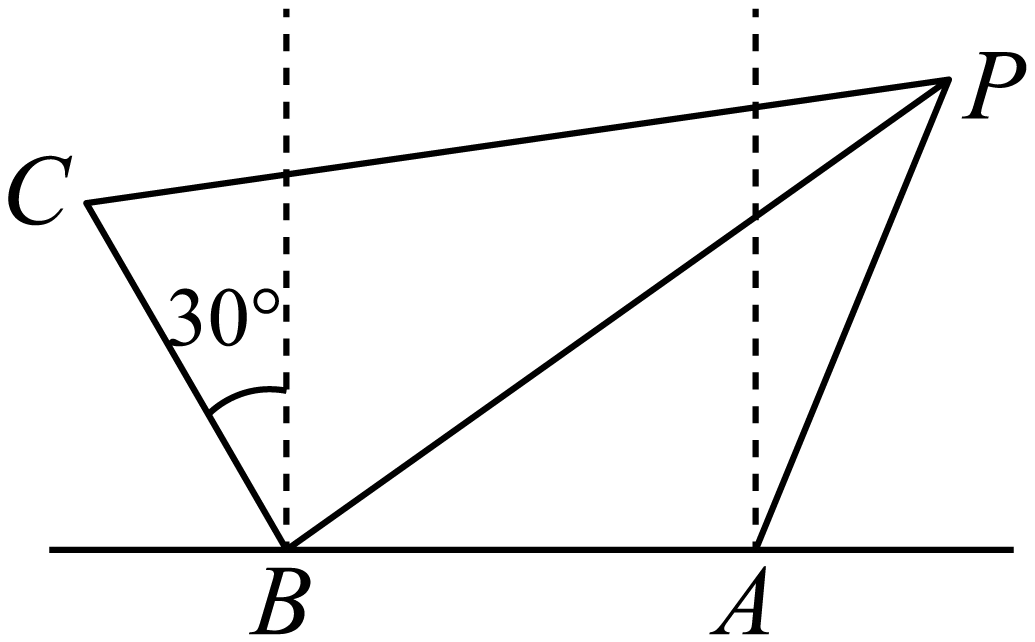
\includegraphics[width=40mm]{figs/14-拓33-13.png}}
\xiexwei{14mm}

{\ansblockgrayfalse
\begin{ansblock}[2章-拓-课时14-33-13]
% ans:2章-拓-课时14-33-13
\ansitem{47}{在 A 的北偏东 30° 方向，相距 10 海里处。}
\ansnote{详解}{以\(AB\)为\(x\)轴、\(AB\)中点为原点建系：\(A(3,0)\)，\(B(-3,0)\)，\(C(-5,2\sqrt{3})\)．\(|PB|-|PA|=4<6=|AB|\)，\(P\)在以\(A\)、\(B\)为焦点、实轴长4的双曲线右支上：\(x^{2}/4-y^{2}/5=1\)（\(x\geqslant 2\)）．\par\noindent \(|PB|=|PC|\)（\(B\)、\(C\)同时收到），\(P\)在\(BC\)中垂线上：\(BC\)中点\((-4,\sqrt{3})\)，\(k_{BC}=2\sqrt{3}/(-5+3)=-\sqrt{3}\)，中垂线\(y-\sqrt{3}=(\sqrt{3}/3)(x+4)\)，即\(x-\sqrt{3}y+7=0\)．与双曲线联立（\(y=(x+7)/\sqrt{3}\)代入）：\(11x^{2}-56x-256=0\)，解得\(x=8\)或\(x=-32/11\)（左支交点，不合\(x\geqslant 2\)，舍），\(y=5\sqrt{3}\)．\(P(8,5\sqrt{3})\)：\(k_{AP}=5\sqrt{3}/(8-3)=\sqrt{3}\)，倾斜角\(60^{\circ}\)，\(|PA|=10\)．故\(P\)在\(A\)的北偏东\(30^{\circ}\)方向，相距10海里处．验算：\(|PB|=\sqrt{11^{2}+75}=14\)，\(|PB|-|PA|=4\)合．}
\end{ansblock}}

\tjdnr{五}{模型求e与实际应用}{例\textbf{48}}{简单(知识点一)}{若椭圆\(x^{2}/9+y^{2}/k^{2}=1\)与双曲线\(x^{2}/k-y^{2}/3=1\)有相同的焦点，则\(k\)的值为\kongbai{}．}
\xiexwei{7mm}

\begin{ansblock}[2章-拓-课时14-34-1]
% ans:2章-拓-课时14-34-1
\ansitem{48}{2}
\ansnote{详解}{两者焦点均在\(x\)轴：\(9-k^{2}=k+3\)（\(k>0\)），即\(k^{2}+k-6=0\)，\((k+3)(k-2)=0\)，\(k=2\)（\(k=-3\)舍）．验算：\(k=2\)时椭圆\(c^{2}=9-4=5\)，双曲线\(c^{2}=2+3=5\)合．}
\end{ansblock}

\liB{变式\textbf{49}}{简单(知识点一)}{}{从某个角度观察篮球（如图1），可以得到一个对称的平面图形，如图2所示，篮球的外轮形状为圆\(O\)，将篮球表面的粘合线看成坐标轴和双曲线，若坐标轴和双曲线与圆\(O\)的交点将圆\(O\)的周长八等分，\(AB=(1/2)BC=CD=1\)，则该双曲线的焦距为\nobreak(\kongwei)}
\ansfig{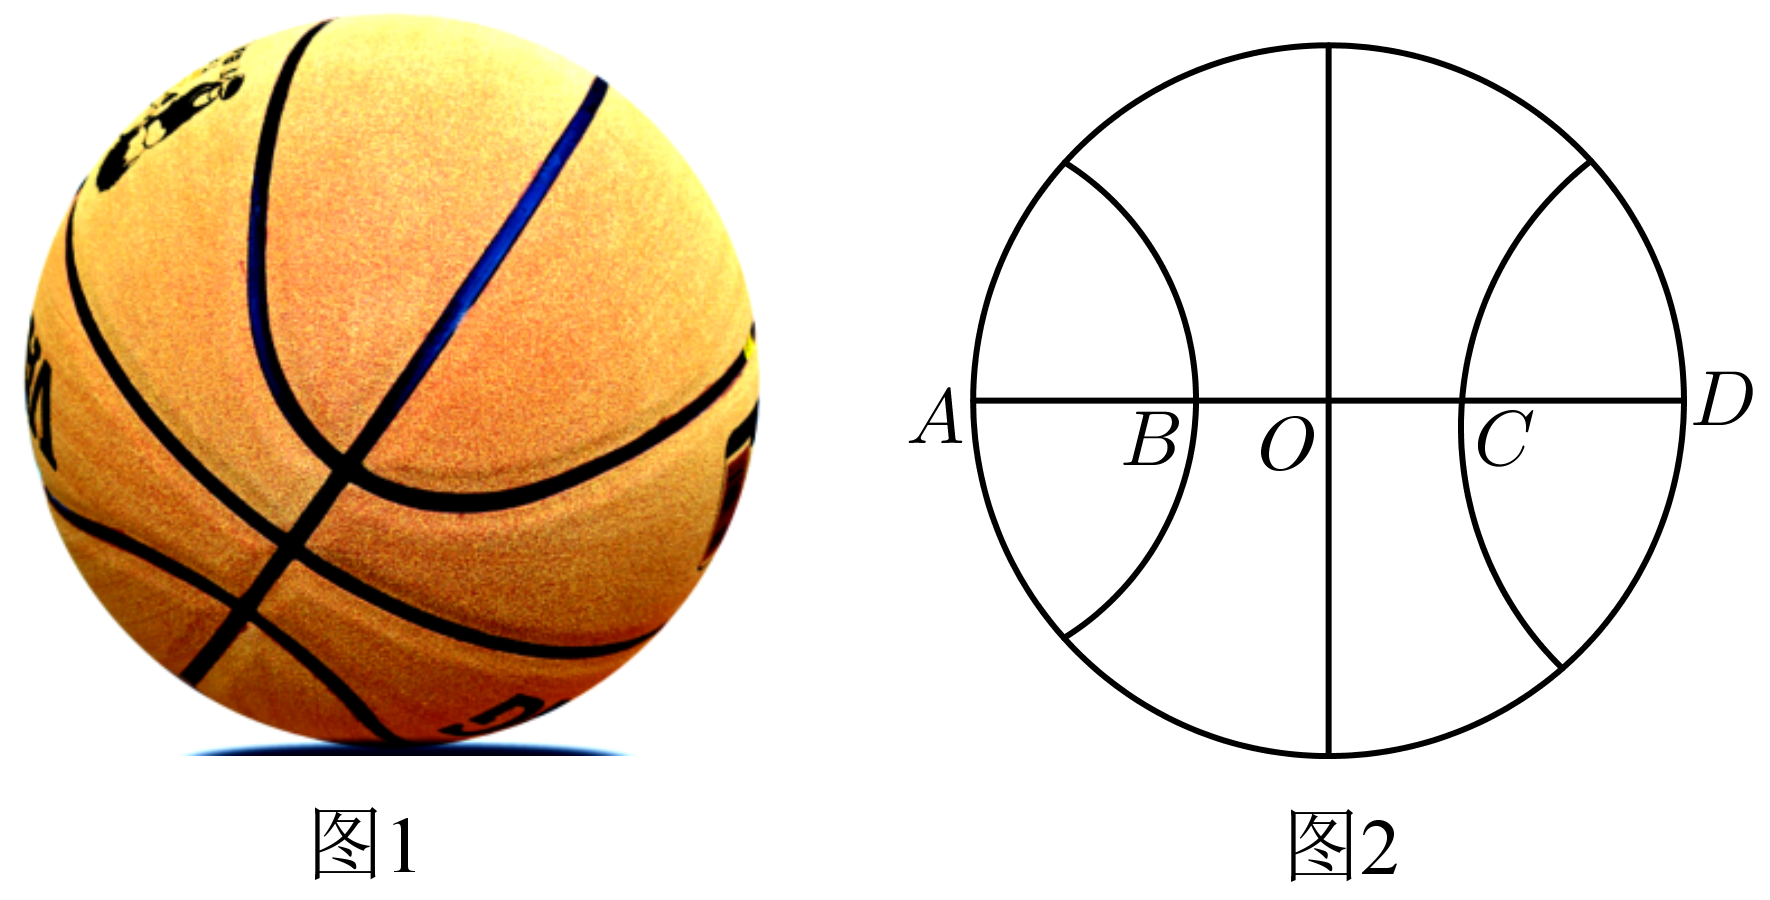
\includegraphics[width=40mm]{figs/14-拓34-2.png}}

\bindopt {\fontsize{10.5pt}{\qpTJgLeadLiti}\selectfont \makebox[\dimexpr0.5\linewidth-1em\relax][l]{A．\(\sqrt{2}\)}\makebox[\dimexpr0.5\linewidth-1em\relax][l]{B．\(\sqrt{6}/2\)}\par}

\bindopt {\fontsize{10.5pt}{\qpTJgLeadLiti}\selectfont \makebox[\dimexpr0.5\linewidth-1em\relax][l]{C．\(2\sqrt{3}\)}\makebox[\dimexpr0.5\linewidth-1em\relax][l]{D．\(4\sqrt{7}/7\)}\par}

\begin{ansblock}[2章-拓-课时14-34-2]
% ans:2章-拓-课时14-34-2
\ansitem{49}{C}
\ansnote{详解}{以\(O\)为原点、\(AD\)所在直线为\(x\)轴建系．八等分结合\(AB=1\)、\(BC=2\)、\(CD=1\)：圆半径\(R=2\)，双曲线过点\((\sqrt{2},\sqrt{2})\)，\(a=1\)．\(2/1-2/b^{2}=1\)，得\(b^{2}=2\)，\(c^{2}=1+2=3\)，\(c=\sqrt{3}\)，焦距\(2\sqrt{3}\)，故选C．}
\end{ansblock}

\liB{变式\textbf{50}}{简单(知识点二)}{}{已知双曲线\(C\)：\(x^{2}/a^{2}-y^{2}/b^{2}=1\)（\(a>0\)，\(b>0\)）的左焦点为\(F_1\)，\(P\)为左支上一点，\(|PF_1|=a\)，\(P_0\)与\(P\)关于原点对称，且\(\overrightarrow{P_0F_1}\cdot\overrightarrow{PF_1}=0\)，则双曲线的渐近线方程为\nobreak(\kongwei)}

\bindopt {\fontsize{10.5pt}{\qpTJgLeadLiti}\selectfont \makebox[\dimexpr0.5\linewidth-1em\relax][l]{A．\(y=\pm x\)}\makebox[\dimexpr0.5\linewidth-1em\relax][l]{B．\(y=\pm(\sqrt{6}/2)x\)}\par}

\bindopt {\fontsize{10.5pt}{\qpTJgLeadLiti}\selectfont \makebox[\dimexpr0.5\linewidth-1em\relax][l]{C．\(y=\pm(\sqrt{3}/2)x\)}\makebox[\dimexpr0.5\linewidth-1em\relax][l]{D．\(y=\pm 2x\)}\par}

\begin{ansblock}[2章-拓-课时14-34-3]
% ans:2章-拓-课时14-34-3
\ansitem{50}{B}
\ansnote{详解}{\(\overrightarrow{P_0F_1}\cdot\overrightarrow{PF_1}=0\)，即\(P_0F_1\perp PF_1\)；\(P_0\)与\(P\)关于原点对称，\(|P_0F_2|=|PF_1|=a\)且\(P_0F_1\perp P_0F_2\)（\(P_0F_2\parallel PF_1\)）．\(P_0\)在右支：\(|P_0F_1|-|P_0F_2|=2a\)，得\(|P_0F_1|=3a\)．Rt\(\triangle P_0F_1F_2\)（直角在\(P_0\)）：\((3a)^{2}+a^{2}=4c^{2}\)，\(10a^{2}=4(a^{2}+b^{2})\)，\(b^{2}/a^{2}=3/2\)．渐近线\(y=\pm(\sqrt{6}/2)x\)，故选B．}
\end{ansblock}

\liB{变式\textbf{51}}{中档(知识点三)}{}{已知点\(M(0,1)\)，点\(P\)是双曲线\(x^{2}/3-y^{2}=1\)上的点，点\(Q\)是点\(P\)关于原点的对称点，则\(\overrightarrow{MP}\cdot\overrightarrow{MQ}\)的取值范围是\kongbai{}．}
\xiexwei{7mm}

\begin{ansblock}[2章-拓-课时14-34-4]
% ans:2章-拓-课时14-34-4
\ansitem{51}{(−∞,−2]}
\ansnote{详解}{设\(P(x_0,y_0)\)（\(|x_0|\geqslant\sqrt{3}\)），\(Q(-x_0,-y_0)\)．\(\overrightarrow{MP}=(x_0,y_0-1)\)，\(\overrightarrow{MQ}=(-x_0,-y_0-1)\)，\(\overrightarrow{MP}\cdot\overrightarrow{MQ}=-x_0^{2}-y_0^{2}+1\)．由\(y_0^{2}=x_0^{2}/3-1\)：\(\overrightarrow{MP}\cdot\overrightarrow{MQ}=-x_0^{2}-x_0^{2}/3+1+1=2-(4/3)x_0^{2}\leqslant 2-(4/3)\times 3=-2\)．取值范围\((- \infty,-2]\)．}
\end{ansblock}

\tjdnr{五}{模型求e与实际应用}{例\textbf{52}}{简单(知识点一)}{已知双曲线\(x^{2}/a^{2}-y^{2}/b^{2}=1\)（\(a>0\)，\(b>0\)）的左、右焦点分别为\(F_1\)，\(F_2\)，点\(P\)在双曲线的右支上，且\(|PF_1|=4|PF_2|\)，求双曲线的离心率\(e\)的最大值．}
\xiexwei{12mm}

\begin{ansblock}[2章-拓-课时14-34-5]
% ans:2章-拓-课时14-34-5
\ansitem{52}{最大值为 5/3。}
\ansnote{详解}{\(|PF_1|-|PF_2|=3|PF_2|=2a\)，得\(|PF_2|=(2/3)a\)．右支焦半径\(|PF_2|\geqslant c-a\)：\((2/3)a\geqslant c-a\)，\(c\leqslant (5/3)a\)，\(e\leqslant 5/3\)；又\(e>1\)．故\(e\)的最大值\(5/3\)．}
\end{ansblock}

\liB{变式\textbf{53}}{简单(知识点一)}{}{南非双曲线大教堂由伦敦著名的建筑事务所完成．若将如图所示的双曲线大教堂外形弧线的一段近似看成双曲线\(y^{2}/a^{2}-x^{2}/b^{2}=1\)（\(a>0\)，\(b>0\)）下支的一部分，且此双曲线过点\((1,-2)\)，离心率为\(\sqrt{6}/2\)，则此双曲线的方程为\nobreak(\kongwei)}
\ansfig{
\includegraphics[width=36mm]{figs/14-拓34-6.png}}

\bindopt {\fontsize{10.5pt}{\qpTJgLeadLiti}\selectfont \makebox[\dimexpr0.5\linewidth-1em\relax][l]{A．\(y^{2}/2-x^{2}=1\)}\makebox[\dimexpr0.5\linewidth-1em\relax][l]{B．\(y^{2}/2-x^{2}/3=1\)}\par}

\bindopt {\fontsize{10.5pt}{\qpTJgLeadLiti}\selectfont \makebox[\dimexpr0.5\linewidth-1em\relax][l]{C．\(y^{2}/2-x^{2}/4=1\)}\makebox[\dimexpr0.5\linewidth-1em\relax][l]{D．\(y^{2}/3-x^{2}/3=1\)}\par}

\begin{ansblock}[2章-拓-课时14-34-6]
% ans:2章-拓-课时14-34-6
\ansitem{53}{A}
\ansnote{详解}{\(e^{2}=3/2=c^{2}/a^{2}=(a^{2}+b^{2})/a^{2}\)，得\(b^{2}=a^{2}/2\)．过\((1,-2)\)：\(4/a^{2}-1/b^{2}=1\)，\(4/a^{2}-2/a^{2}=1\)，\(a^{2}=2\)，\(b^{2}=1\)．方程\(y^{2}/2-x^{2}=1\)，故选A．验算：\(4/2-1/1=1\)合，\(e=\sqrt{3/2}=\sqrt{6}/2\)合．}
\end{ansblock}

\xiaojie{①识别：以通径、正六边形、蒙日圆、共轭双曲线、焦点三角形、矩形对角线等为载体的求离心率模型题，以及时差定位、扫描半径、花瓶截面等实际应用题，判归本题型.}
\bindp {\kaishu ②操作：几何模型先译成\(a\)、\(b\)、\(c\)的齐次等式再同除\(a^{2}\)（或\(a\)）化\(e\)的方程；应用题建系—定义—定\(a\)、\(c\)—写方程（带范围）—回问作答.}
\bindp {\kaishu ③收束：\(e\)的方程注意\(e>1\)的取根范围；范围题盯住端点与取等条件；应用题最后一步必须回到实际量纲（方向角、距离、单位）.}

% ---------- 探究点六 定点定值压轴 ----------
\tjdnr{六}{定点定值压轴}{例\textbf{54}}{难(知识点三)}{已知双曲线\(C\)：\(x^{2}/4-y^{2}=1\)．(1)求双曲线\(C\)的离心率；(2)若直线\(l\)：\(y=kx+m\)与双曲线\(C\)相交于\(A\)，\(B\)两点（\(A\)，\(B\)均异于左、右顶点），且以\(AB\)为直径的圆过双曲线\(C\)的左顶点\(D\)，求证：直线\(l\)过定点，并求出该定点的坐标．}
\xiexwei{18mm}

{\ansblockgrayfalse
\begin{ansblock}[2章-练-课时14-15]
% ans:2章-练-课时14-15
\ansitem{54}{(1) e=√5/2；(2) 证明见解析，定点坐标为 (−10/3,0)。}
\ansnote{详解}{(1)\(a=2\)，\(b=1\)，\(c=\sqrt{4+1}=\sqrt{5}\)，\(e=c/a=\sqrt{5}/2\)．\par\noindent (2)设\(A(x_1,y_1)\)，\(B(x_2,y_2)\)．联立\(y=kx+m\)与\(x^{2}/4-y^{2}=1\)：\((1-4k^{2})x^{2}-8mkx-4(m^{2}+1)=0\)，其中\(1-4k^{2}\neq 0\)（否则\(l\)与渐近线平行，不合两交点），\(\Delta=64m^{2}k^{2}+16(1-4k^{2})(m^{2}+1)>0\)；\(x_1+x_2=8mk/(1-4k^{2})\)，\(x_1x_2=-4(m^{2}+1)/(1-4k^{2})\)；\(y_1y_2=(kx_1+m)(kx_2+m)=k^{2}x_1x_2+mk(x_1+x_2)+m^{2}=(m^{2}-4k^{2})/(1-4k^{2})\)．\par\noindent 以\(AB\)为直径的圆过\(D(-2,0)\Leftrightarrow\overrightarrow{DA}\cdot\overrightarrow{DB}=0\Leftrightarrow(x_1+2)(x_2+2)+y_1y_2=0\)，即\(x_1x_2+2(x_1+x_2)+4+y_1y_2=0\)．通分（分母\(1-4k^{2}\)）：\([m^{2}-4k^{2}]+[-4(m^{2}+1)]+[16mk]+[4(1-4k^{2})]=-3m^{2}+16mk-20k^{2}=0\)，即\(3m^{2}-16mk+20k^{2}=0\)，解得\(m=2k\)或\(m=(10/3)k\)．\par\noindent 当\(m=2k\)时，\(l\)：\(y=k(x+2)\)过\(D(-2,0)\)，此时\(A\)、\(B\)之一即\(D\)，与“\(A\)、\(B\)均异于左、右顶点”矛盾，舍去；当\(m=(10/3)k\)时（\(k\neq 0\)），\(l\)：\(y=k(x+10/3)\)恒过定点\((-10/3,0)\)，且不过\(D\)，符合题意．故直线\(l\)过定点，定点坐标为\((-10/3,0)\)．验算：\(3m^{2}-16mk+20k^{2}=(3m-10k)(m-2k)\)合；定点\((-10/3,0)\)在左顶点\(D(-2,0)\)左侧，直线族绕该点转动时与双曲线恒有两交点（\(k\)充分小时），满足\(\Delta>0\)合．}
\end{ansblock}}

\liB{变式\textbf{55}}{难(知识点三)}{}{设\(F_1\)，\(F_2\)是双曲线\(C\)：\(x^{2}/a^{2}-y^{2}/b^{2}=1\)（\(a>0\)，\(b>0\)）的左、右两个焦点，\(O\)为坐标原点，若点\(P\)在双曲线\(C\)的右支上，且\(|OP|=|OF_1|=2\)，\(\triangle PF_1F_2\)的面积为3．(1)求双曲线\(C\)的渐近线方程；(2)若双曲线\(C\)的两顶点分别为\(A_1(-a,0)\)，\(A_2(a,0)\)，过点\(F_2\)的直线\(l\)与双曲线\(C\)交于\(M\)，\(N\)两点，试探究直线\(A_1M\)与直线\(A_2N\)的交点\(Q\)是否在某条定直线上？若在，请求出该定直线方程；若不在，请说明理由．}
\xiexwei{18mm}

{\ansblockgrayfalse
\begin{ansblock}[2章-练-课时14-16]
% ans:2章-练-课时14-16
\ansitem{55}{(1) y=±√3x；(2) 存在，定直线方程 x=1/2。}
\ansnote{详解}{(1)\(|OF_1|=|OF_2|=c=2\)，\(|OP|=|OF_1|\)说明\(\triangle PF_1F_2\)中边\(F_1F_2\)上的中线等于该边一半，故\(\angle F_1PF_2=90^{\circ}\)，即\(PF_1\perp PF_2\)．\(P\)在右支：\(|PF_1|-|PF_2|=2a\)；面积：\(|PF_1|\cdot|PF_2|=2S=6\)．\(|PF_1|^{2}+|PF_2|^{2}=|F_1F_2|^{2}=(2c)^{2}=16=(|PF_1|-|PF_2|)^{2}+2|PF_1||PF_2|=4a^{2}+12\)，得\(4a^{2}=4\)，\(a=1\)．\(b^{2}=c^{2}-a^{2}=4-1=3\)，渐近线\(y=\pm(b/a)x=\pm\sqrt{3}x\)．\par\noindent (2)双曲线\(C\)：\(x^{2}-y^{2}/3=1\)．（i）\(l\)斜率不存在：\(l\)：\(x=2\)，\(M(2,3)\)，\(N(2,-3)\)．直线\(A_1M\)：\(y=x+1\)；直线\(A_2N\)：\(y=-3x+3\)．联立得\(Q(1/2,3/2)\)，横坐标\(1/2\)．\par\noindent （ii）\(l\)斜率存在：\(l\)过\(F_2(2,0)\)且不与渐近线平行，设\(l\)：\(y=k(x-2)\)（\(k\neq 0\)，\(k\neq\pm\sqrt{3}\)），\(M(x_1,y_1)\)，\(N(x_2,y_2)\)．联立得\((3-k^{2})x^{2}+4k^{2}x-4k^{2}-3=0\)，\(x_1+x_2=4k^{2}/(k^{2}-3)\)，\(x_1x_2=(4k^{2}+3)/(k^{2}-3)\)．直线\(A_1M\)：\(y=[y_1/(x_1+1)](x+1)\)；直线\(A_2N\)：\(y=[y_2/(x_2-1)](x-1)\)．交点\(Q(x,y)\)满足\((x+1)/(x-1)=y_2(x_1+1)/[y_1(x_2-1)]\)（\(x\neq 1\)）．两边平方，以\(y_1^{2}=3(x_1^{2}-1)\)、\(y_2^{2}=3(x_2^{2}-1)\)代入：\([(x+1)/(x-1)]^{2}=[3(x_2^{2}-1)(x_1+1)^{2}]/[3(x_1^{2}-1)(x_2-1)^{2}]=[(x_2+1)(x_1+1)]/[(x_1-1)(x_2-1)]=[x_1x_2+(x_1+x_2)+1]/[x_1x_2-(x_1+x_2)+1]=[(4k^{2}+3)+4k^{2}+(k^{2}-3)]/[(4k^{2}+3)-4k^{2}+(k^{2}-3)]=9k^{2}/k^{2}=9\)．故\((x+1)/(x-1)=\pm 3\)，得\(x=1/2\)或\(x=2\)．\par\noindent 取\(x=2\)需\(y_2(x_1+1)/[y_1(x_2-1)]=+3>0\)；但\(M\)、\(N\)是过右焦点的弦的两端点且均非顶点：\(0<k^{2}<3\)时\(M\)、\(N\)分居两支（\(x_1x_2<0\)），\(x_2-1<0\)而\(y_1y_2>0\)；\(k^{2}>3\)时\(M\)、\(N\)同在右支且分居\(x\)轴两侧，\(y_1y_2<0\)而\((x_1+1)(x_2-1)>0\)——两种情形该式恒为负，只能取\(-3\)．故\(x=2\)为平方增根，舍去，\(x=1/2\)．综上，交点\(Q\)恒在定直线\(x=1/2\)上．验算：（i）的\(Q(1/2,3/2)\)落在\(x=1/2\)上合；（ii）韦达分子分母化简\(4k^{2}+3+4k^{2}+k^{2}-3=9k^{2}\)、\(4k^{2}+3-4k^{2}+k^{2}-3=k^{2}\)，比值9合．}
\end{ansblock}}

\tjdnr{六}{定点定值压轴}{例\textbf{56}}{难(知识点三)}{双曲线\(C\)：\(x^{2}-y^{2}/2=1\)，过定点\(A(-1,0)\)的两条互相垂直的直线分别交双曲线于\(P\)、\(Q\)两点，直线\(PQ\)恒过定点\nobreak(\kongwei)}

\bindopt {\fontsize{10.5pt}{\qpTJgLeadLiti}\selectfont \makebox[\dimexpr0.5\linewidth-1em\relax][l]{A．\((1,0)\)}\makebox[\dimexpr0.5\linewidth-1em\relax][l]{B．\((2,0)\)}\par}

\bindopt {\fontsize{10.5pt}{\qpTJgLeadLiti}\selectfont \makebox[\dimexpr0.5\linewidth-1em\relax][l]{C．\((3,0)\)}\makebox[\dimexpr0.5\linewidth-1em\relax][l]{D．\((4,0)\)}\par}

{\ansblockgrayfalse
\begin{ansblock}[2章-拓-课时14-28]
% ans:2章-拓-课时14-28
\ansitem{56}{C}
\ansnote{详解}{设\(PQ\)：\(x=my+b\)，联立\(x^{2}-y^{2}/2=1\)：\((m^{2}-1/2)y^{2}+2bmy+b^{2}-1=0\)．设\(P(x_1,y_1)\)，\(Q(x_2,y_2)\)：\(y_1+y_2=-2bm/(m^{2}-1/2)\)，\(y_1y_2=(b^{2}-1)/(m^{2}-1/2)\)．\(AP\perp AQ\)（\(A(-1,0)\)）：\((x_1+1)(x_2+1)+y_1y_2=0\)，以\(x_i=my_i+b\)代入：\((1+m^{2})y_1y_2+(b+1)m(y_1+y_2)+(b+1)^{2}=0\)．\par\noindent 通分（乘\(m^{2}-1/2\)）：\(2(b^{2}-1)(1+m^{2})-4bm^{2}(b+1)+(2m^{2}-1)(b+1)^{2}=0\)．按\(m\)整理——\(m^{2}\)系数：\(2(b^{2}-1)-4b(b+1)+2(b+1)^{2}=2b^{2}-2-4b^{2}-4b+2b^{2}+4b+2=0\)（恒为0）；常数项：\(2(b^{2}-1)-(b+1)^{2}=b^{2}-2b-3=0\)，得\(b=3\)或\(b=-1\)．\(b=-1\)时\(PQ\)过\(A(-1,0)\)（\(P\)、\(Q\)之一与\(A\)重合或直线退化），舍去；\(b=3\)，\(PQ\)恒过\((3,0)\)．故选C．\par\noindent 验算（特例）：\(PQ\perp x\)轴即\(m=0\)、\(x=3\)：与\(x^{2}-y^{2}/2=1\)交于\((3,\pm 4)\)；\(\overrightarrow{AP}=(4,4)\)、\(\overrightarrow{AQ}=(4,-4)\)，\(\overrightarrow{AP}\cdot\overrightarrow{AQ}=16-16=0\)合．}
\end{ansblock}}

\liB{变式\textbf{57}}{难(知识点三)}{}{已知双曲线\(C\)：\(x^{2}/a^{2}-y^{2}/b^{2}=1\)（\(a>0\)，\(b>0\)）的右焦点为\(F(c,0)\)，离心率为2，直线\(x=a^{2}/c\)与双曲线\(C\)的一条渐近线交于点\(P\)，且\(|PF|=\sqrt{3}\)．(1)求双曲线\(C\)的标准方程；(2)设\(Q\)为双曲线右支上的一个动点，证明：在\(x\)轴的负半轴上存在定点\(M\)，使得\(\angle QFM=2\angle QMF\)．}
\xiexwei{18mm}

{\ansblockgrayfalse
\begin{ansblock}[2章-拓-课时14-29]
% ans:2章-拓-课时14-29
\ansitem{57}{(1) x²−y²/3=1；(2) 证明见解析，M(−1,0)。}
\ansnote{详解}{(1)取渐近线\(y=(b/a)x\)，与\(x=a^{2}/c\)交于\(P(a^{2}/c,ab/c)\)．\(|PF|^{2}=(c-a^{2}/c)^{2}+(ab/c)^{2}\)，其中\(c-a^{2}/c=(c^{2}-a^{2})/c=b^{2}/c\)，故\(|PF|^{2}=b^{4}/c^{2}+a^{2}b^{2}/c^{2}=b^{2}(a^{2}+b^{2})/c^{2}=b^{2}c^{2}/c^{2}=b^{2}\)．由\(|PF|=\sqrt{3}\)得\(b^{2}=3\)．\(e^{2}=c^{2}/a^{2}=4=(a^{2}+b^{2})/a^{2}\)，得\(a^{2}=1\)．\(C\)：\(x^{2}-y^{2}/3=1\)．\par\noindent (2)\(F(2,0)\)．设\(Q(x_0,y_0)\)（\(x_0\geqslant 1\)），\(3x_0^{2}-y_0^{2}=3\)．①\(x_0=2\)时\(y_0=\pm 3\)：\(\angle QFM=90^{\circ}\)需\(\angle QMF=45^{\circ}\)，\(|MF|=|QF|=|y_0|=3\)，得\(M(-1,0)\)，符合．②\(x_0\neq 2\)时设\(M(t,0)\)（\(t<0\)）．有向正切：\(\tan\angle QFM=-y_0/(x_0-2)\)，\(\tan\angle QMF=y_0/(x_0-t)\)．\(\angle QFM=2\angle QMF\)，由倍角公式：\(-y_0/(x_0-2)=2[y_0/(x_0-t)]/(1-[y_0/(x_0-t)]^{2})\)．\(y_0\neq 0\)时约去\(y_0\)、交叉相乘：\(-[(x_0-t)^{2}-y_0^{2}]=2(x_0-2)(x_0-t)\)，展开整理：\(3x_0^{2}-y_0^{2}-(4+4t)x_0+4t+t^{2}=0\)．以\(3x_0^{2}-y_0^{2}=3\)代入：\(-(4+4t)x_0+(t^{2}+4t+3)=0\)，对任意\(x_0\geqslant 1\)（\(x_0\neq 2\)）恒成立，故\(-(4+4t)=0\)且\(t^{2}+4t+3=0\)，得\(t=-1\)（两式公共解）．\(y_0=0\)（\(Q\)为右顶点）时直接验证\(M(-1,0)\)亦满足\(\angle QFM=2\angle QMF\)．综上，存在定点\(M(-1,0)\)．验算：\(t^{2}+4t+3=(t+1)(t+3)\)与\(-(4+4t)\)公共根\(t=-1\)合；取\(Q(2,3)\)：\(\angle QFM=90^{\circ}\)、\(\angle QMF=45^{\circ}\)，\(2\times 45^{\circ}=90^{\circ}\)合．}
\end{ansblock}}

\liB{变式\textbf{58}}{难(知识点三)}{}{已知\(F_1(-2,0)\)，\(F_2(2,0)\)，点\(P\)满足\(|PF_1|-|PF_2|=2\)，记点\(P\)的轨迹为\(\Gamma\)．斜率为\(k\)的直线\(l\)过点\(F_2\)，且与轨迹\(\Gamma\)相交于\(A\)，\(B\)两点．(1)求轨迹\(\Gamma\)的方程；(2)求斜率\(k\)的取值范围；(3)在\(x\)轴上是否存在定点\(M\)，使得无论直线\(l\)绕点\(F_2\)怎样转动，总有\(MA\perp MB\)成立？如果存在，求出定点\(M\)；如果不存在，请说明理由．}
\xiexwei{18mm}

{\ansblockgrayfalse
\begin{ansblock}[2章-拓-课时14-30]
% ans:2章-拓-课时14-30
\ansitem{58}{(1) x²−y²/3=1（x>0）；(2) (−∞,−√3)∪(√3,+∞)；(3) 存在，M(−1,0)。}
\ansnote{详解}{(1)\(|PF_1|-|PF_2|=2<|F_1F_2|=4\)，轨迹为以\(F_1\)、\(F_2\)为焦点、实轴长2的双曲线右支：\(c=2\)，\(a=1\)，\(b^{2}=3\)，\(\Gamma\)：\(x^{2}-y^{2}/3=1\)（\(x>0\)）．\par\noindent (2)\(l\)：\(y=k(x-2)\)，代入\(\Gamma\)：\((3-k^{2})x^{2}+4k^{2}x-4k^{2}-3=0\)．\(A\)、\(B\)为两交点（右支上\(x>0\)）：需\(3-k^{2}\neq 0\)、\(\Delta>0\)、\(x_1+x_2=-4k^{2}/(3-k^{2})>0\)、\(x_1x_2=(-4k^{2}-3)/(3-k^{2})>0\)．由\(x_1+x_2>0\)得\(k^{2}>3\)；此时\(x_1x_2>0\)、\(\Delta=16k^{4}-4(3-k^{2})(-4k^{2}-3)>0\)亦成立．故\(k\in(-\infty,-\sqrt{3})\cup(\sqrt{3},+\infty)\)．\par\noindent (3)存在性：设\(M(m,0)\)．\(l\)与\(\Gamma\)联立同上：\((3-k^{2})x^{2}+4k^{2}x-4k^{2}-3=0\)（\(k^{2}>3\)），\(x_1+x_2=-4k^{2}/(3-k^{2})\)，\(x_1x_2=(-4k^{2}-3)/(3-k^{2})\)．\(MA\perp MB\Leftrightarrow(x_1-m)(x_2-m)+y_1y_2=0\)，\(y_i=k(x_i-2)\)：\((1+k^{2})x_1x_2-(m+2k^{2})(x_1+x_2)+m^{2}+4k^{2}=0\)．乘\((3-k^{2})\)展开：\((1+k^{2})(-4k^{2}-3)+4k^{2}(2k^{2}+m)+(m^{2}+4k^{2})(3-k^{2})=0\)，即\(k^{2}(-m^{2}+4m+5)+3m^{2}-3=0\)，对一切\(k^{2}>3\)恒成立．故\(-m^{2}+4m+5=0\)且\(3m^{2}-3=0\)，得\(m=-1\)（\(m=1\)不满足第一式）．斜率不存在时\(l\)：\(x=2\)，\(A(2,3)\)、\(B(2,-3)\)：\(\overrightarrow{MA}=(3,3)\)、\(\overrightarrow{MB}=(3,-3)\)，\(\overrightarrow{MA}\cdot\overrightarrow{MB}=0\)合．综上，存在\(M(-1,0)\)．验算：\(k^{2}(-m^{2}+4m+5)+3m^{2}-3\)在\(m=-1\)时两项恒为0合；(3)的韦达代入式与(2)一致合．}
\end{ansblock}}

\tjdnr{六}{定点定值压轴}{例\textbf{59}}{中档(知识点三)}{已知双曲线\(x^{2}/a^{2}-y^{2}/b^{2}=1\)（\(a>0\)，\(b>0\)）的左、右焦点分别为\(F_1\)，\(F_2\)，点\(P\)在双曲线的右支上，\(|PF_1|\)，\(|PF_2|\)的最小值\(m_1\)，\(m_2\)，且满足\(m_1m_2=3a^{2}\)．(1)求双曲线的离心率；(2)若\(a=2\)，过点\(F_1\)的直线交双曲线于\(A\)，\(B\)两点，线段\(AB\)的垂直平分线交\(y\)轴于点\(D\)（异于坐标原点\(O\)），求\(|AB|/|OD|\)的最小值．}
\xiexwei{18mm}

{\ansblockgrayfalse
\begin{ansblock}[2章-拓-课时14-33-4]
% ans:2章-拓-课时14-33-4
\ansitem{59}{(1) e=2；(2) 3/2。}
\ansnote{详解}{(1)右支上\(|PF_1|_{\min}=c+a\)（左顶点处），\(|PF_2|_{\min}=c-a\)（右顶点处）．\(m_1m_2=c^{2}-a^{2}=b^{2}=3a^{2}\)，得\(c^{2}=4a^{2}\)，\(e=2\)．\par\noindent (2)\(a=2\)，\(c=4\)，\(b^{2}=12\)，双曲线\(x^{2}/4-y^{2}/12=1\)，\(F_1(-4,0)\)．设\(AB\)：\(y=k(x+4)\)（\(k\neq\pm\sqrt{3}\)）．联立：\((3-k^{2})x^{2}-8k^{2}x-16k^{2}-12=0\)，\(x_1+x_2=8k^{2}/(3-k^{2})\)，\(x_1x_2=(-16k^{2}-12)/(3-k^{2})\)．弦长\(|AB|=\sqrt{1+k^{2}}\cdot\sqrt{(x_1+x_2)^{2}-4x_1x_2}=12(1+k^{2})/|3-k^{2}|\)．中点\((4k^{2}/(3-k^{2}),12k/(3-k^{2}))\)（\(y_1+y_2=k(x_1+x_2)+8k=24k/(3-k^{2})\)）．垂直平分线：\(y-12k/(3-k^{2})=-(1/k)(x-4k^{2}/(3-k^{2}))\)，令\(x=0\)得\(y=16k/(3-k^{2})\)，\(|OD|=16|k|/|3-k^{2}|\)．\par\noindent \(|AB|/|OD|=[12(1+k^{2})/|3-k^{2}|]\cdot[|3-k^{2}|/(16|k|)]=(3/4)(|k|+1/|k|)\geqslant 3/2\)（\(|k|=1\)取等），最小值\(3/2\)．验算：\((x_1-x_2)^{2}=(8k^{2}/(3-k^{2}))^{2}+4(16k^{2}+12)/(3-k^{2})=[64k^{4}+4(16k^{2}+12)(3-k^{2})]/(3-k^{2})^{2}=144(k^{2}+1)/(3-k^{2})^{2}\)，\(|AB|=\sqrt{1+k^{2}}\cdot 12\sqrt{k^{2}+1}/|3-k^{2}|\)合．}
\end{ansblock}}

\liB{变式\textbf{60}}{中档(知识点三)}{}{已知双曲线的离心率为\(\sqrt{6}/2\)，且该双曲线经过点\(P(\sqrt{3},\sqrt{2}/2)\)．(1)求双曲线\(C\)：\(x^{2}/a^{2}-y^{2}/b^{2}=1\)（\(a>0\)，\(b>0\)）的方程；(2)设斜率分别为\(k_1\)，\(k_2\)的两条直线\(l_1\)，\(l_2\)均经过点\(Q(2,1)\)，且直线\(l_1\)，\(l_2\)与双曲线\(C\)分别交于\(A\)，\(B\)两点（\(A\)，\(B\)异于点\(Q\)），若\(k_1+k_2=1\)，试判断直线\(AB\)是否经过定点，若存在定点，求出该定点坐标；若不存在，说明理由。}
\xiexwei{18mm}

{\ansblockgrayfalse
\begin{ansblock}[2章-拓-课时14-33-5]
% ans:2章-拓-课时14-33-5
\ansitem{60}{(1) x²/2−y²=1；(2) 过定点 (0,1)。}
\ansnote{详解}{(1)\(e^{2}=3/2=c^{2}/a^{2}=(a^{2}+b^{2})/a^{2}\)，得\(b^{2}/a^{2}=1/2\)，即\(a^{2}=2b^{2}\)，双曲线方程为\(x^{2}/(2b^{2})-y^{2}/b^{2}=1\)．代入\(P\)：\(3/(2b^{2})-(1/2)/b^{2}=1\)，\((3-1)/(2b^{2})=1\)，\(b^{2}=1\)，\(a^{2}=2\)．\(C\)：\(x^{2}/2-y^{2}=1\)．\par\noindent (2)\(AB\)斜率不存在时：\(A(x_0,y_0)\)、\(B(x_0,-y_0)\)，\(k_1+k_2=(y_0-1)/(x_0-2)+(-y_0-1)/(x_0-2)=-2/(x_0-2)=1\)，得\(x_0=0\)，不在曲线上，舍；故斜率存在．设\(AB\)：\(y=kx+t\)，代入：\((2k^{2}-1)x^{2}+4ktx+2t^{2}+2=0\)（\(2k^{2}-1\neq 0\)），\(x_1+x_2=-4kt/(2k^{2}-1)\)，\(x_1x_2=(2t^{2}+2)/(2k^{2}-1)\)．\par\noindent \(k_1+k_2=1\)：\((kx_1+t-1)/(x_1-2)+(kx_2+t-1)/(x_2-2)=1\)，即\((2k-1)x_1x_2+(t-2k+1)(x_1+x_2)-4t=0\)．代入：\((2k-1)(2t^{2}+2)-4kt(t-2k+1)-4t(2k^{2}-1)=0\)（通分后乘\(2k^{2}-1\)），整理\(t^{2}+(2k-2)t-1+2k=0\)，即\((t-1)(t+2k-1)=0\)．\(t=1\)：\(y=kx+1\)过\((0,1)\)；\(t=1-2k\)：\(y=k(x-2)+1\)过\(Q(2,1)\)，不合（\(A\)、\(B\)异于\(Q\)且\(Q\)为弦端情形）．故直线\(AB\)过定点\((0,1)\)．验算：\(t^{2}+(2k-2)t+2k-1=(t-1)(t+2k-1)\)展开核对合．}
\end{ansblock}}

\liB{变式\textbf{61}}{中档(知识点三)}{}{已知双曲线\(C\)过点\((4,\sqrt{3})\)，且渐近线方程为\(y=\pm(1/2)x\)，直线\(l\)与曲线\(C\)交于点\(M\)、\(N\)两点．(1)求双曲线\(C\)的方程；(2)若直线\(l\)过点\((1,0)\)，问在\(x\)轴上是否存在定点\(Q\)，使得\(\overrightarrow{QM}\cdot\overrightarrow{QN}\)为常数？若存在，求出点坐标及此常数的值；若不存在，说明理由。}
\xiexwei{18mm}

{\ansblockgrayfalse
\begin{ansblock}[2章-拓-课时14-33-6]
% ans:2章-拓-课时14-33-6
\ansitem{61}{(1) x²/4−y²=1；(2) 存在，Q(23/8,0)，QM·QN=273/64。}
\ansnote{详解}{(1)\(b/a=1/2\)且\(16/a^{2}-3/b^{2}=1\)：\(b^{2}=a^{2}/4\)，\(16/a^{2}-12/a^{2}=1\)，\(a^{2}=4\)，\(b^{2}=1\)．\(C\)：\(x^{2}/4-y^{2}=1\)．\par\noindent (2)设\(l\)：\(x=my+1\)，联立：\((m^{2}-4)y^{2}+2my-3=0\)（\(m^{2}\neq 4\)，\(\Delta>0\)得\(m^{2}>3\)），\(y_1+y_2=-2m/(m^{2}-4)\)，\(y_1y_2=-3/(m^{2}-4)\)；\(x_1+x_2=m(y_1+y_2)+2=-8/(m^{2}-4)\)，\(x_1x_2=(my_1+1)(my_2+1)=-(4m^{2}+4)/(m^{2}-4)\)．设\(Q(t,0)\)：\(\overrightarrow{QM}\cdot\overrightarrow{QN}=(x_1-t)(x_2-t)+y_1y_2=x_1x_2-t(x_1+x_2)+t^{2}+y_1y_2=-4+t^{2}+(8t-23)/(m^{2}-4)\)．与\(m\)无关\(\Leftrightarrow 8t-23=0\)，得\(t=23/8\)，常数\(-4+t^{2}=-4+529/64=273/64\)．验算：\(x_1x_2=(-4m^{2}-4)/(m^{2}-4)=-4-20/(m^{2}-4)\)；三项合并分子\(-20-3+8t=8t-23\)，故数量积\(-4+t^{2}+(8t-23)/(m^{2}-4)\)合．}
\end{ansblock}}

\liB{变式\textbf{62}}{中档(知识点三)}{}{设直线\(2x-y+1=0\)与椭圆\(x^{2}/3+y^{2}/4=1\)相交于\(A\)、\(B\)两点．(1)求弦长\(|AB|\)；(2)已知椭圆具有性质：设\(A\)、\(B\)为椭圆\(x^{2}/a^{2}+y^{2}/b^{2}=1\)上任意两点，\(M\)是线段\(AB\)的中点，若直线\(AB\)、\(OM\)的斜率都存在，并记为\(k_{AB}\)、\(k_{OM}\)，则\(k_{AB}\cdot k_{OM}\)为定值．试对双曲线\(x^{2}/a^{2}-y^{2}/b^{2}=1\)写出具有类似特征的性质，并加以证明．}
\xiexwei{18mm}

{\ansblockgrayfalse
\begin{ansblock}[2章-拓-课时14-33-7]
% ans:2章-拓-课时14-33-7
\catcode`\_=12\relax
\ansitem{62}{(1) 15/4；(2) 双曲线中 k_AB·k_OM=b²/a²（定值），证明见解析。}
\catcode`\_=8\relax
\ansnote{详解}{(1)联立得\(16x^{2}+12x-9=0\)，\(x_1+x_2=-3/4\)，\(x_1x_2=-9/16\)．根差\((x_1-x_2)^{2}=(-3/4)^{2}-4\times(-9/16)=45/16\)，故\(|AB|=\sqrt{5}\cdot 3\sqrt{5}/4=15/4\)．\par\noindent (2)性质：双曲线\(x^{2}/a^{2}-y^{2}/b^{2}=1\)上任意两点\(A\)、\(B\)（斜率存在时），\(M\)为\(AB\)中点，则\(k_{AB}\cdot k_{OM}=b^{2}/a^{2}\)．证明（点差法）：\(A(x_3,y_3)\)、\(B(x_4,y_4)\)、\(M(x_0,y_0)\)．两式相减：\((x_3+x_4)(x_3-x_4)/a^{2}=(y_3+y_4)(y_3-y_4)/b^{2}\)，即\(2x_0(x_3-x_4)/a^{2}=2y_0(y_3-y_4)/b^{2}\)，变形得\(k_{AB}\cdot k_{OM}=[(y_3-y_4)/(x_3-x_4)]\cdot(y_0/x_0)=b^{2}/a^{2}\)．定值证毕．验算：\(k_{AB}\cdot k_{OM}=b^{2}/a^{2}\)与例24的\(k_1k_2=b^{2}/a^{2}\)相容（中心对称两点为其特例）合．}
\end{ansblock}}

\liB{变式\textbf{63}}{中档(知识点三)}{}{已知双曲线\(C\)：\(x^{2}/a^{2}-y^{2}/b^{2}=1\)（\(a>0\)，\(b>0\)）的一个焦点坐标为\((3,0)\)，其中一条渐近线的倾斜角的正切值为\(2\sqrt{2}\)，\(O\)为坐标原点．(1)求双曲线\(C\)的方程；(2)直线\(l\)与\(x\)轴正半轴相交于一点\(D\)，与双曲线\(C\)右支相切（切点不为右顶点），且\(l\)分别交双曲线\(C\)的两条渐近线于\(M\)、\(N\)两点，证明：\(\triangle MON\)的面积为定值，并求出该定值．}
\xiexwei{18mm}

{\ansblockgrayfalse
\begin{ansblock}[2章-拓-课时14-33-8]
% ans:2章-拓-课时14-33-8
\ansitem{63}{(1) x²−y²/8=1；(2) 定值 2√2。}
\ansnote{详解}{(1)\(c=3\)，\(b/a=2\sqrt{2}\)，\(a^{2}+b^{2}=9\)，得\(a^{2}(1+8)=9\)，\(a^{2}=1\)，\(b^{2}=8\)．\(C\)：\(x^{2}-y^{2}/8=1\)．\par\noindent (2)\(l\)：\(y=kx+m\)（\(k\neq\pm 2\sqrt{2}\)，\(m\neq 0\)，斜率存在且不为0）．\(D(-m/k,0)\)，\(|OD|=|m/k|\)．相切：联立\((8-k^{2})x^{2}-2kmx-m^{2}-8=0\)，\(\Delta=0\)，得\(4k^{2}m^{2}+4(8-k^{2})(m^{2}+8)=0\)，即\(m^{2}=k^{2}-8\)（\(k^{2}>8\)）．\(M\)与\(y=2\sqrt{2}x\)交：\((m/(2\sqrt{2}-k),2\sqrt{2}m/(2\sqrt{2}-k))\)；\(N\)与\(y=-2\sqrt{2}x\)交：\((-m/(2\sqrt{2}+k),2\sqrt{2}m/(2\sqrt{2}+k))\)．\(S_{\triangle MON}=S_{\triangle MOD}+S_{\triangle NOD}=(1/2)|OD|\cdot|y_M-y_N|=(1/2)|m|\cdot|x_M-x_N|=(1/2)|m|\cdot|4\sqrt{2}m/(8-k^{2})|=2\sqrt{2}m^{2}/(k^{2}-8)=2\sqrt{2}\)（定值）．验算：\(m^{2}=k^{2}-8>0\)与\(k^{2}>8\)一致合；\(S\)只依赖\(m^{2}/(k^{2}-8)\)，化简后为常数合．}
\end{ansblock}}

\liB{变式\textbf{64}}{中档(知识点三)}{}{已知双曲线\(\Gamma\)：\(x^{2}/a^{2}-y^{2}/b^{2}=1\)（\(a>0\)，\(b>0\)）的左、右顶点分别为\(A_1(-1,0)\)、\(A_2(1,0)\)，离心率为2，过点\(F(2,0)\)斜率不为0的直线\(l\)与\(\Gamma\)交于\(P\)、\(Q\)两点．(1)求双曲线\(\Gamma\)的渐近线方程；(2)记直线\(A_1P\)、\(A_2Q\)的斜率分别为\(k_1\)、\(k_2\)，求证：\(k_1/k_2\)为定值．}
\xiexwei{18mm}

{\ansblockgrayfalse
\begin{ansblock}[2章-拓-课时14-33-9]
% ans:2章-拓-课时14-33-9
\ansitem{64}{(1) y=±√3x；(2) 定值 k₁/k₂=−1/3。}
\ansnote{详解}{(1)\(a=1\)，\(c=2\)，\(b^{2}=3\)，\(\Gamma\)：\(x^{2}-y^{2}/3=1\)，渐近线\(y=\pm\sqrt{3}x\)．\par\noindent (2)\(l\)斜率不存在：\(P(2,3)\)、\(Q(2,-3)\)，\(k_1=3/3=1\)、\(k_2=-3/1=-3\)，比值\(-1/3\)．\(l\)：\(y=k(x-2)\)（\(k\neq 0\)）：\((k^{2}-3)x^{2}-4k^{2}x+4k^{2}+3=0\)，\(x_1+x_2=4k^{2}/(k^{2}-3)\)，\(x_1x_2=(4k^{2}+3)/(k^{2}-3)\)．\(3k_1+k_2=3y_1/(x_1+1)+y_2/(x_2-1)=k[4x_1x_2-5(x_1+x_2)+4]/[(x_1+1)(x_2-1)]\)．\(4x_1x_2-5(x_1+x_2)+4=[4(4k^{2}+3)-20k^{2}+4(k^{2}-3)]/(k^{2}-3)=0\)．故\(3k_1+k_2=0\)，\(k_1/k_2=-1/3\)（定值），综上得证．验算：分子\(16k^{2}+12-20k^{2}+4k^{2}-12=0\)合．}
\end{ansblock}}

\liB{变式\textbf{65}}{中档(知识点三)}{}{设双曲线\(x^{2}/a^{2}-y^{2}/b^{2}=1\)，其虚轴长为\(2\sqrt{2}\)，且离心率为\(\sqrt{5}\)．(1)求双曲线\(C\)的方程；(2)过点\(P(3,1)\)的动直线与双曲线的左右两支曲线分别交于点\(A\)、\(B\)，在线段\(AB\)上取点\(M\)使得\(|AM|/|MB|=|AP|/|PB|\)，证明：点\(M\)落在某一定直线上．}
\xiexwei{18mm}

{\ansblockgrayfalse
\begin{ansblock}[2章-拓-课时14-33-10]
% ans:2章-拓-课时14-33-10
\ansitem{65}{(1) 2x²−y²/2=1；(2) 定直线 12x−y−2=0。}
\ansnote{详解}{(1)\(2b=2\sqrt{2}\)，得\(b^{2}=2\)；\(e^{2}=5=1+b^{2}/a^{2}\)，得\(a^{2}=1/2\)．\(C\)：\(2x^{2}-y^{2}/2=1\)．\par\noindent (2)设\(M(x,y)\)、\(A(x_1,y_1)\)、\(B(x_2,y_2)\)（\(x_1<x_2<3\)）．\(|AM|/|MB|=|AP|/|PB|\)结合共线定比：\((3-x_1)/(x_2-3)=-(x-x_1)/(x_2-x)\)，即\([6-(x_1+x_2)]x=3(x_1+x_2)-2x_1x_2\)．①设\(l\)：\(y-1=k(x-3)\)，代入\(C\)：\((4-k^{2})x^{2}+(6k^{2}-2k)x-9k^{2}+6k-3=0\)，\(x_1+x_2=(2k-6k^{2})/(4-k^{2})\)，\(x_1x_2=(-9k^{2}+6k-3)/(4-k^{2})\)．代入①整理：\(12x-3=k(x-3)\)，与\(y-1=k(x-3)\)联立消\(k\)：\(12x-3=y-1\)，即\(12x-y-2=0\)．点\(M\)恒落在定直线\(12x-y-2=0\)上．验算：由定比\(x=[3(x_1+x_2)-2x_1x_2]/[6-(x_1+x_2)]\)（分比不变）合；韦达代入化简得\(12x-3=k(x-3)\)，代回\(y-1=k(x-3)\)消\(k\)得\(y=12x-2\)合．}
\end{ansblock}}

\liB{变式\textbf{66}}{中档(知识点三)}{}{已知\(A\)，\(B\)分别是双曲线\(E\)：\(x^{2}-y^{2}/4=1\)的左，右顶点，直线\(l\)（不与坐标轴垂直）过点\(N(2,0)\)，且与双曲线\(E\)交于\(C\)，\(D\)两点．(1)若\(|CN|=3|ND|\)，求直线\(l\)的方程；(2)若直线\(AC\)与\(BD\)相交于点\(P\)，求证：点\(P\)在定直线上．}
\xiexwei{18mm}

{\ansblockgrayfalse
\begin{ansblock}[2章-拓-课时14-33-11]
% ans:2章-拓-课时14-33-11
\ansitem{66}{(1) 2√5x−y−4√5=0 或 2√5x+y−4√5=0；(2) 定直线 x=1/2。}
\ansnote{详解}{设\(l\)：\(x=my+2\)，\(C(x_1,y_1)\)、\(D(x_2,y_2)\)，联立：\((4m^{2}-1)y^{2}+16my+12=0\)，\(y_1+y_2=-16m/(4m^{2}-1)\)，\(y_1y_2=12/(4m^{2}-1)\)．\par\noindent (1)\(|CN|=3|ND|\)（\(N\)为\(F_2\)，\(C\)、\(D\)同向分段），得\(y_1=-3y_2\)，\(y_2=8m/(4m^{2}-1)\)；代入\(y_1y_2=-3y_2^{2}=12/(4m^{2}-1)\)：\(-3\times 64m^{2}/(4m^{2}-1)^{2}=12/(4m^{2}-1)\)，得\(-16m^{2}=4m^{2}-1\)，\(m^{2}=1/20\)，\(m=\pm\sqrt{5}/10\)．直线\(l\)：\(x=\pm(\sqrt{5}/10)y+2\)，即\(2\sqrt{5}x-y-4\sqrt{5}=0\)或\(2\sqrt{5}x+y-4\sqrt{5}=0\)．\par\noindent (2)\(AC\)：\(y=[y_1/(x_1+1)](x+1)\)；\(BD\)：\(y=[y_2/(x_2-1)](x-1)\)．以\(x_1=my_1+2\)、\(x_2=my_2+2\)代入，得\(x_1+1=my_1+3\)、\(x_2-1=my_2+1\)．联立：\((x+1)/(x-1)=(my_1y_2+3y_2)/(my_1y_2+y_1)\)．由韦达\(y_1y_2=12/(4m^{2}-1)\)、\(y_1+y_2=-16m/(4m^{2}-1)\)，得\(y_1y_2=-[3/(4m)](y_1+y_2)\)．于是\((x+1)/(x-1)=[-(3/4)(y_1+y_2)+3y_2]/[-(3/4)(y_1+y_2)+y_1]=(-3y_1+9y_2)/(y_1-3y_2)=-3\)，解得\(x=1/2\)．点\(P\)恒在定直线\(x=1/2\)上．验算：\((-3y_1+9y_2)/(y_1-3y_2)=-3(y_1-3y_2)/(y_1-3y_2)=-3\)合；(1)中\(-16m^{2}=4m^{2}-1\)即\(20m^{2}=1\)合．}
\end{ansblock}}

\xiaojie{①识别：以定点、定值、定直线为设问的综合压轴题（弦恒过定点、交点恒在定线、比值与面积定值），判归本题型；基本路径是“设线—联立—韦达—把几何约束化为系数恒等式”.}
\bindp {\kaishu ②操作：垂直、等比、面积等约束经韦达代入化成\(x_1+x_2\)、\(x_1x_2\)的恒等式，令参数系数为零解出定点（值）；平方取根、退化情形（直线过顶点、与渐近线平行、弦端重合）须逐一检验舍.}
\bindp {\kaishu ③收束：过焦点/定点的弦可设\(x=my+b\)绕开斜率不存在情形；结论用特例（水平弦、垂直弦）快速自检；定点若与题设排除点重合即为增根.}

% ============================================================
% 课堂评价 G5（恒5＝3单选+2填空＝导槽 G1~G5；ketang 新制顺排可跨栏，禁 \vbox 装栏）
% 印面号 67—71
% ============================================================
\begin{ketang}{本组共5题（第67—71题），67—69为单选，70—71为填空．}

\jiancestem{{\fontsize{11.4pt}{14pt}\selectfont\heihao {\numboldjian 67}．}\hspace{4.1mm}\tieside{简单(知识点一)}\hspace{2.2mm}已知双曲线\(C\)：\(x^{2}/9-y^{2}/m=1\)（\(m>0\)）的离心率为\(\sqrt{13}/3\)，则\(C\)的渐近线方程为\nobreak(\kongwei)}

\bindopt {\fontsize{10.5pt}{\qpTJgLeadPingjia}\selectfont \makebox[\dimexpr0.5\linewidth-1em\relax][l]{A．\(y=\pm(2/3)x\)}\makebox[\dimexpr0.5\linewidth-1em\relax][l]{B．\(y=\pm(3/2)x\)}\par}

\bindopt {\fontsize{10.5pt}{\qpTJgLeadPingjia}\selectfont \makebox[\dimexpr0.5\linewidth-1em\relax][l]{C．\(y=\pm\sqrt{3}x\)}\makebox[\dimexpr0.5\linewidth-1em\relax][l]{D．\(y=\pm(\sqrt{13}/3)x\)}\par}

\begin{ansblock}[2章-导-课时14-G1]
% ans:2章-导-课时14-G1
\ansitem{67}{A}
\ansnote{详解}{\(e^{2}=1+b^{2}/a^{2}=1+m/9=13/9\)，得\(m/9=4/9\)，\(m=4\)．故\(C\)：\(x^{2}/9-y^{2}/4=1\)，\(a=3\)、\(b=2\)，渐近线\(y=\pm(b/a)x=\pm(2/3)x\)，选A．验算：\(e=\sqrt{1+4/9}=\sqrt{13}/3\)合．}
\end{ansblock}

\jiancestem{{\fontsize{11.4pt}{14pt}\selectfont\heihao {\numboldjian 68}．}\hspace{4.1mm}\tieside{简单(知识点二)}\hspace{2.2mm}渐近线方程为\(y=\pm(\sqrt{2}/2)x\)，且焦点在\(x\)轴上的双曲线的标准方程可以是\nobreak(\kongwei)}

\bindopt {\fontsize{10.5pt}{\qpTJgLeadPingjia}\selectfont \makebox[\dimexpr0.5\linewidth-1em\relax][l]{A．\(x^{2}/4-y^{2}/2=1\)}\makebox[\dimexpr0.5\linewidth-1em\relax][l]{B．\(y^{2}/2-x^{2}/4=1\)}\par}

\bindopt {\fontsize{10.5pt}{\qpTJgLeadPingjia}\selectfont \makebox[\dimexpr0.5\linewidth-1em\relax][l]{C．\(x^{2}/2-y^{2}/4=1\)}\makebox[\dimexpr0.5\linewidth-1em\relax][l]{D．\(y^{2}/4-x^{2}/16=1\)}\par}

\begin{ansblock}[2章-导-课时14-G2]
% ans:2章-导-课时14-G2
\ansitem{68}{A}
\ansnote{详解}{逐项核两条件：A：\(a^{2}=4\)、\(b^{2}=2\)，渐近线\(y=\pm(b/a)x=\pm(\sqrt{2}/2)x\)，\(c^{2}=4+2=6\)，焦点\((\pm\sqrt{6},0)\)在\(x\)轴，两条件皆合；B：渐近线\(y=\pm(a/b)x=\pm(\sqrt{2}/2)x\)与A相同，但实轴在\(y\)轴上，焦点\((0,\pm\sqrt{6})\)，不合“焦点在\(x\)轴”；C：渐近线\(y=\pm(b/a)x=\pm\sqrt{2}x\)，不合；D：渐近线\(y=\pm(a/b)x=\pm(1/2)x\)且焦点\((0,\pm 2\sqrt{5})\)在\(y\)轴，两条件皆不合．故选A．}
\end{ansblock}

\jiancestem{{\fontsize{11.4pt}{14pt}\selectfont\heihao {\numboldjian 69}．}\hspace{4.1mm}\tieside{中档(知识点一)}\hspace{2.2mm}已知双曲线\(C\)：\(x^{2}/a^{2}-y^{2}/b^{2}=1\)（\(a>0\)，\(b>0\)）的离心率\(e\in[\sqrt{3},2]\)，则\(b/a\)的取值范围为\nobreak(\kongwei)}

\bindopt {\fontsize{10.5pt}{\qpTJgLeadPingjia}\selectfont \makebox[\dimexpr0.5\linewidth-1em\relax][l]{A．\([\sqrt{2},\sqrt{3}]\)}\makebox[\dimexpr0.5\linewidth-1em\relax][l]{B．\([1,\sqrt{3}]\)}\par}

\bindopt {\fontsize{10.5pt}{\qpTJgLeadPingjia}\selectfont \makebox[\dimexpr0.5\linewidth-1em\relax][l]{C．\([\sqrt{3},2]\)}\makebox[\dimexpr0.5\linewidth-1em\relax][l]{D．\([2,3]\)}\par}

\begin{ansblock}[2章-导-课时14-G3]
% ans:2章-导-课时14-G3
\ansitem{69}{A}
\ansnote{详解}{由\(e^{2}=1+(b/a)^{2}\)得\((b/a)^{2}=e^{2}-1\)．\(e\in[\sqrt{3},2]\)，则\(e^{2}\in[3,4]\)，\((b/a)^{2}\in[2,3]\)；又\(b/a>0\)，故\(b/a\in[\sqrt{2},\sqrt{3}]\)，选A．验算：\(e=\sqrt{3}\)时\(b/a=\sqrt{2}\)，\(e=2\)时\(b/a=\sqrt{3}\)，端点可取合．}
\end{ansblock}

\jiancestem{{\fontsize{11.4pt}{14pt}\selectfont\heihao {\numboldjian 70}．}\hspace{4.1mm}\tieside{简单(知识点二)}\hspace{2.2mm}已知双曲线的焦点在\(x\)轴上，虚轴长为4，渐近线方程为\(y=\pm(1/2)x\)，则该双曲线的标准方程为\kongbai{}．}
\xiexwei{7mm}

\begin{ansblock}[2章-导-课时14-G4]
% ans:2章-导-课时14-G4
\ansitem{70}{x²/16−y²/4=1}
\ansnote{详解}{虚轴长\(2b=4\)，得\(b=2\)；焦点在\(x\)轴时渐近线为\(y=\pm(b/a)x\)，由\(b/a=1/2\)得\(a=2b=4\)．故标准方程为\(x^{2}/16-y^{2}/4=1\)．验算：\(a^{2}=16\)、\(b^{2}=4\)，渐近线\(y=\pm(2/4)x=\pm(1/2)x\)合，虚轴\(2b=4\)合，\(c^{2}=20\)，焦点\((\pm 2\sqrt{5},0)\)在\(x\)轴合．}
\end{ansblock}

\jiancestem{{\fontsize{11.4pt}{14pt}\selectfont\heihao {\numboldjian 71}．}\hspace{4.1mm}\tieside{中档(知识点二)}\hspace{2.2mm}已知双曲线\(C_1\)：\(x^{2}/2-y^{2}/m=1\)（\(m>0\)）与双曲线\(C_2\)：\(x^{2}-y^{2}/7=1\)的渐近线相同，则\(m=\)\kongbai{}，\(C_1\)的离心率为\kongbai{}．}
\xiexwei{7mm}

\begin{ansblock}[2章-导-课时14-G5]
% ans:2章-导-课时14-G5
\ansitem{71}{m=14；e=2√2}
\ansnote{详解}{\(C_2\)（\(a^{2}=1\)、\(b^{2}=7\)）的渐近线为\(y=\pm\sqrt{7}x\)．\(C_1\)（\(a^{2}=2\)、\(b^{2}=m\)，焦点同在\(x\)轴）的渐近线为\(y=\pm(\sqrt{m}/\sqrt{2})x\)．渐近线相同即\(\sqrt{m}/\sqrt{2}=\sqrt{7}\)，得\(\sqrt{m}=\sqrt{14}\)，\(m=14\)．此时\(e^{2}=1+b^{2}/a^{2}=1+14/2=8\)，故\(e=2\sqrt{2}\)．验算：\(m=14\)时\(C_1\)渐近线\(y=\pm(\sqrt{14}/\sqrt{2})x=\pm\sqrt{7}x\)合，\(e=\sqrt{8}=2\sqrt{2}\)合．}
\end{ansblock}

\end{ketang}

% ---- 尾块（\tailfill 置 \end{multicols} 前；无参＝内容尾随框，件侧不擅自定高） ----
\tailfill

\end{multicols}
\end{document}
